%  LaTeX support: latex@mdpi.com
%=================================================================
% Fix for older pdfTeX / xcolor incompatibility
% \PassOptionsToPackage{dvips}{xcolor}  % removed: conflicts with pdftex driver
\documentclass[fire,article,submit,pdftex]{../Definitions/mdpi}

% Additional packages
% ---------------------------------------------------------------
% Submission source of truth for the Fire manuscript package.
% Final figure and table assets follow the numbering used in the paper.
% ---------------------------------------------------------------
\usepackage[utf8]{inputenc}
\usepackage{graphicx}
\setlength{\headheight}{20.0pt}
\addtolength{\topmargin}{-8.0pt}
\usepackage{amsmath,amssymb}
% Prevent widow/orphan lines and improve float placement
\widowpenalty=10000
\clubpenalty=10000
\brokenpenalty=4991
% Unicode characters that may appear in SVG text layers
\DeclareUnicodeCharacter{2264}{$\leq$}%   ≤
\DeclareUnicodeCharacter{2265}{$\geq$}%   ≥
\DeclareUnicodeCharacter{2212}{$-$}%      − (minus sign)
\DeclareUnicodeCharacter{00D7}{$\times$}% ×
\DeclareUnicodeCharacter{03B1}{$\alpha$}% α
\DeclareUnicodeCharacter{03B2}{$\beta$}%  β
\usepackage{booktabs}
\usepackage{multirow}
\usepackage{siunitx}
% \usepackage{algorithmic}  % removed: not used in this manuscript
% \usepackage{algorithm}    % removed: not used in this manuscript

% Pagination and metadata
\firstpage{1}
\makeatletter
\setcounter{page}{\@firstpage}
\makeatother
\pubvolume{1}
\issuenum{1}
\articlenumber{0}
\pubyear{2026}
\copyrightyear{2026}
\datereceived{ }
\daterevised{ }
\dateaccepted{ }
\datepublished{ }

%=================================================================
\Title{A Survival--Probability Fusion Prototype for Censor-Aware Multi-Horizon Wildfire Threat Forecasting and Decision-Utility Evaluation}

\Author{Zhengyang Ren $^{1,*}$}
\AuthorNames{Zhengyang Ren}

\address{%
$^{1}$ \quad Jiaying University, 100 Meisong Road, Meijiang District, Meizhou 514015, Guangdong, China; d58350215@gmail.com}

\corres{Correspondence: d58350215@gmail.com}

%=================================================================
\abstract{%
For emergency managers facing an advancing wildfire, the question that drives evacuation timing is not simply \emph{whether} fire will arrive but \emph{how soon}. Current prediction tools tend to ignore right censoring, neglect probability coherence across successive time windows, or skip calibration altogether---shortcomings that limit their operational value.
We present a survival--probability fusion prototype whose backbone is an XGBoost accelerated failure time (AFT) model. On top of this backbone the pipeline attaches horizon-specific probability heads, applies beta calibration, and imposes a monotone fusion constraint, ultimately delivering coherent threat probabilities at the 12, 24, and 48~h marks for individual wildfire--zone encounters.
All training and testing relied on 221 labelled observations (69 events, 152 censored) from the WiDS Datathon 2026 dataset, evaluated through nested five-fold cross-validation with inner cross-fitting. We did not attempt external or incident-grouped validation; every metric reported here derives from internal out-of-fold evaluation only.
The prototype achieved an Uno's IPCW C-index of 0.941 (95\% bootstrap CI 0.924--0.959) and a mean Brier score across the 12, 24, and 48~h horizons of 0.041. Among the three horizons, 24~h stood out as best calibrated (slope~= 0.998), with risk terciles exhibiting strong separation (observed event rates: 0.0\%, 4.5\%, 92.3\%). At the 24--48~h boundary, roughly one quarter of observations needed monotone correction.
We also conducted a frank comparison against simpler alternatives. At the present events-per-variable ratio ($\approx$~2.0), a Random Survival Forest yielded lower probability error and better seed-to-seed stability, and stripped-down AFT variants reproduced the full prototype's discrimination with far fewer moving parts. The full architecture should therefore be read as a methodological proof of concept; its added complexity will only pay off once substantially more data become available.
}

\keyword{wildfire forecasting; evacuation risk; survival analysis; censoring; multi-horizon prediction; calibration; risk stratification; monotone fusion; decision curve analysis}

%%%%%%%%%%%%%%%%%%%%%%%%%%%%%%%%%%%%%%%%%%
\begin{document}
%%%%%%%%%%%%%%%%%%%%%%%%%%%%%%%%%%%%%%%%%%

\section{Introduction}\label{sec:introduction}

Managing wildfire risk today demands more than a binary ``will fire arrive'' forecast---what practitioners actually need is a probabilistic picture of \emph{when} a fire will threaten each evacuation zone.
The reason timing is so central is straightforward: horizon-specific threat probabilities feed directly into which zones get evacuated first, where suppression crews and equipment are staged, and when alerts go out to residents~\cite{Finney2001,Xi2019,Stephens2018}.
Large wildfires have grown more frequent, more intense, and wider in footprint across both the western United States and other fire-prone regions over the last twenty years~\cite{Jain2022,Cunningham2024,Turco2023,Luo2024,Jones2022,Kolden2024,Higuera2021}, amplifying the urgency for calibrated, multi-horizon tools that go beyond crude distance-based heuristics~\cite{Radeloff2023,Tonini2020}.

Earlier work on predicting wildfire threat can be grouped, roughly, into three camps.
First, physics-informed estimated-time-of-arrival (ETA) models~\cite{Finney2001,Cruz2003} back-calculate when fire will reach a zone from distance and spread rate. This approach is intuitive, but it produces only point estimates and has no built-in way to deal with right-censored observations---cases where monitoring stopped before fire arrival could be confirmed or excluded.
A second stream of research trains single-horizon classifiers that output a binary ``threatened / not-threatened'' label for one fixed time window~\cite{Jaafari2019,Gigovic2019,Chen2024wui}. These classifiers discard information from censored cases and, because each window is modelled independently, there is nothing forcing the predicted probabilities to be consistent from one horizon to the next.
The third camp---survival analysis methods such as Cox proportional-hazards models, accelerated failure time (AFT) regressions, and their machine-learning descendants---handles censoring by construction and yields survival curves whose cumulative incidence values $P(T \leq h)$ are automatically monotone~\cite{Wiegrebe2024,Taylor2013}. Yet when separate horizon-specific classifiers are stacked on top, or when the raw survival CDF is poorly calibrated, the outputs can still drift away from observed event rates and need post-hoc correction~\cite{VanCalster2019}.

Three practical shortcomings hold back current methods in operational evacuation contexts.
The most obvious is that right-censored observations---ubiquitous in wildfire encounter data---are routinely thrown away, injecting survivorship bias. Small labelled samples, which are the norm in this domain, make the problem worse by demanding especially careful cross-validation and regularisation~\cite{Steyerberg2019,Collins2024,Riley2020}.
A second gap concerns cross-horizon consistency. Any operational decision-support tool should ensure that probability estimates at successive horizons (say 12, 24, 48~h) satisfy $P(T \leq 12) \leq P(T \leq 24) \leq P(T \leq 48)$---an obvious monotonicity requirement that classifiers trained horizon-by-horizon regularly violate.
Third, even models with excellent discrimination can produce predicted probabilities that diverge substantially from observed event rates; in other words, absolute calibration matters for threshold-based evacuation rules, not merely ranking~\cite{VanCalster2019}.

Our goal was to construct a survival--probability fusion framework that tackles all three of these gaps at once.
We deliberately chose a small dataset---221 wildfire--zone encounters, only 69 of which are observed events---to stress-test how each module of the pipeline behaves when data are scarce. Given so few events relative to the number of features, we did not expect the full multi-module system to outperform simpler baselines on every metric. Rather, we wanted to show how the components interlock and, equally importantly, to pin down where a leaner model is the more appropriate choice.
In concrete terms, this paper offers three contributions:
\begin{enumerate}
    \item A censor-aware pipeline linking an AFT survival backbone to horizon-specific probability heads, beta calibration, and a monotone fusion layer. The result is a set of coherent 12, 24, and 48~h threat probabilities, each serving a distinct operational role: 24~h turned out to be the best-calibrated horizon, most relevant for staging decisions; 12~h ranks zones effectively but resists precise calibration; and 48~h is useful for longer-lead planning yet more sensitive to censoring assumptions. Roughly 25\% of observations needed monotone correction at the 24--48~h boundary;
    \item A nested cross-validation protocol with inner cross-fitting that separates meta-feature generation from fusion weight estimation, guarding against information leakage;
    \item A head-to-head comparison against simpler alternatives---a Random Survival Forest and stripped-down AFT variants---showing that, at the present events-per-variable ratio, these simpler models match or beat the full architecture on standard metrics. We view this negative result as equally informative for practitioners working under similar data constraints.
\end{enumerate}

\section{Materials and Methods}\label{sec:methods}

\subsection{Study Design and Data Source}\label{sec:data}

This work is a retrospective predictive modelling study.
We obtained the dataset from the WiDS Datathon 2026 wildfire prediction competition; it draws on records from real wildfire incidents across the western United States.
Each row in the dataset represents one \emph{fire--zone pair}---a single wildfire event matched with a single evacuation zone---described by spatio-temporal and dynamic fire-behaviour variables derived from fire perimeter observations collected during the first five hours post-ignition.
Throughout the study, the fire--zone pair is the analysis unit, and every pair contributes one observation.
The labelled portion of the data contains 221 such pairs spanning 37 variables: 69 are events (fire approached within 5~km of the evacuation-zone centroid) and 152 are right-censored (monitoring stopped before fire arrival or the fire was contained).
A separate test set of 95 observations (35 variables) existed but carried no outcome labels, so all model building and evaluation were performed on the 221-observation training partition via nested cross-validation.
Every predictor was available at or before the close of the five-hour observation window, ruling out information leakage from future time points.

\subsection{Outcome Definition and Censoring}\label{sec:outcome}

We define the outcome as the elapsed time, measured in hours, from the end of the five-hour observation window until the fire perimeter crosses within 5~km of the evacuation-zone centroid.
This definition mirrors the WiDS Datathon 2026 task: input features capture fire behaviour during the first five hours after ignition, and the prediction target asks whether the fire breaches the 5~km radius within 12, 24, or 48~h of the observation window's end (Figure~\ref{fig:timeline}).
An observation is right-censored whenever monitoring ceases---because the fire was contained, the observation window lapsed, or for other administrative reasons---before the 5~km threshold is reached.
Censoring due to fire containment is unlikely to be fully non-informative, because containment is an active intervention linked to fire behaviour covariates rather than a random stopping mechanism, which departs from the textbook assumption of independent right censoring~\cite{Steyerberg2019}.

\begin{figure}[!ht]
\centering
    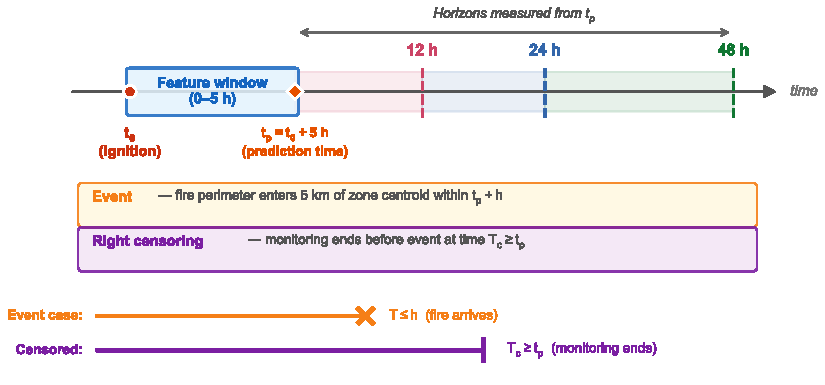
\includegraphics[width=\linewidth]{figures/main/Figure_1_prediction_timeline.pdf}
\caption{Prediction timeline. Features are extracted from the first five hours after ignition ($t_0$). The prediction time $t_p = t_0 + 5$~h defines the origin for all horizons. The event is defined as the fire perimeter entering within 5~km of the evacuation-zone centroid. Observations are right-censored if monitoring ends before the event occurs. An ``$\times$'' denotes an observed event (fire arrival within the horizon); a vertical bar ``$|$'' denotes right censoring (monitoring terminated before the event).}\label{fig:timeline}
\end{figure}

We selected three prediction horizons---12~h, 24~h, and 48~h---to cover the time window most relevant for evacuation logistics: 12~h captures the urgent near-term alert zone, 24~h aligns with typical pre-evacuation lead times, and 48~h is intended for medium-range resource staging~\cite{Stephens2018,Taylor2013}.
A 72~h horizon was also computed, but every eligible observation experienced the event (positive rate = 100\%), rendering the horizon uninformative; 72~h results appear only in Supplementary Materials (Table~S1).

For each horizon $h$, we constructed censor-aware binary labels as follows.
An observation qualifies as \emph{eligible} at horizon $h$ if it either experienced an event at any time or was censored at a time no earlier than $h$.
Within this eligible set, $Y_h = 1$ when the event occurred at time $T \leq h$ and $Y_h = 0$ otherwise.
Observations censored before $h$---whose true status at $h$ cannot be determined---are excluded.
One downside of this binary setup is that it draws no distinction between a fire arriving at $T$ marginally beyond $h$ and a clearly non-threatened zone; a continuous-time competing-risks model could capture this nuance in future extensions.
Eligible sample sizes and positive rates per horizon appear in Table~\ref{tab:horizons}.

\begin{table}[!ht]
\caption{Censor-aware target characteristics for each prediction horizon.}\label{tab:horizons}
\begin{tabular}{lccc}
\toprule
\textbf{Horizon} & \textbf{Eligible $n$} & \textbf{Positives} & \textbf{Positive Rate (\%)} \\
\midrule
12~h  & 215 & 49  & 22.8 \\
24~h  & 196 & 63  & 32.1 \\
48~h  & 166 & 66  & 39.8 \\
72~h$^\dagger$ & 69  & 69  & 100.0 \\
\bottomrule
\multicolumn{4}{l}{\footnotesize $^\dagger$Degenerate; confined to Supplementary Materials.}
\end{tabular}
\end{table}

\subsection{Predictors and Feature Engineering}\label{sec:features}

We organised input features into four conceptual groups:

\paragraph{Distance and urgency features.}
The raw distance to the nearest fire perimeter was re-expressed in three forms: log-distance ($\log(1 + d)$), inverse distance ($1 / (1000 + d)$), and an exponential short-range urgency score ($\exp(-d / 2500)$).
We also computed an estimated time of arrival as $\text{ETA} = d / \max(v_{\mathrm{closing}}, 50)$, capped at 240~h.

\paragraph{Speed and alignment features.}
We retained closing speed (both signed and absolute), centroid speed, and an alignment score that quantifies the angular match between fire spread direction and the vector pointing toward the zone boundary.
A directional push interaction, $\max(v_{\mathrm{closing}}, 0) \times |\text{alignment}|$, was added.

\paragraph{Growth and spread dynamics.}
This group covers area growth rate (ha/h), radial growth rate (m/h), log-transformed growth ($\log(1 + \text{growth})$), and two interaction terms: closing speed $\times$ log-growth and area growth rate $\times$ alignment.

\paragraph{Temporal and regime features.}
Event start hour (period = 24), day of week (period = 7), and month (period = 12) were encoded cyclically via sine/cosine pairs.
Three binary regime flags were defined from distance cutoffs: \emph{threat} ($d < 4500$~m), \emph{boundary} ($4500 \leq d \leq 7000$~m), and \emph{far} ($d > 7000$~m).
These cutoffs are pragmatic rather than definitive. The 4500~m value sits within the range where ember lofting and spot-fire ignition have been documented under moderate-to-high wind in coniferous fuel types~\cite{Cruz2003,Finney2001}; 7000~m roughly matches outer perimeters used for pre-evacuation staging in California~\cite{Dolan2022}. Both should be regarded as engineering rules of thumb whose suitability will vary with fuel type and terrain.
For the ETA calculation, closing speed was floored at 50~m/h (a conservative bound for slow ground fires) and the resulting arrival time was capped at 240~h (10~days), past which the forecast has little operational relevance~\cite{Taylor2013}.

Altogether, the feature set consists of 26 engineered variables plus 8 columns retained from the original dataset (after removing identifiers and outcome fields), for a total of 34 modelling features (the full dictionary is in Supplementary Table~S0).
We applied median imputation for continuous predictors and mode imputation for binary flags, done separately within each outer training fold so that validation data never informed the fill values; as it turned out, no variable in the analysed dataset actually contained missing entries (Supplementary Table~S11), so this step was precautionary rather than corrective.
A ``thin'' variant limited to the 26 engineered features was tested in the ablation study to gauge how much the retained original columns contribute.

\subsection{Proposed Framework}\label{sec:model}

The proposed framework consists of four modules (Figure~\ref{fig:framework}):

\begin{figure}[!ht]
\begin{adjustwidth}{-\extralength}{0cm}
    \centering
    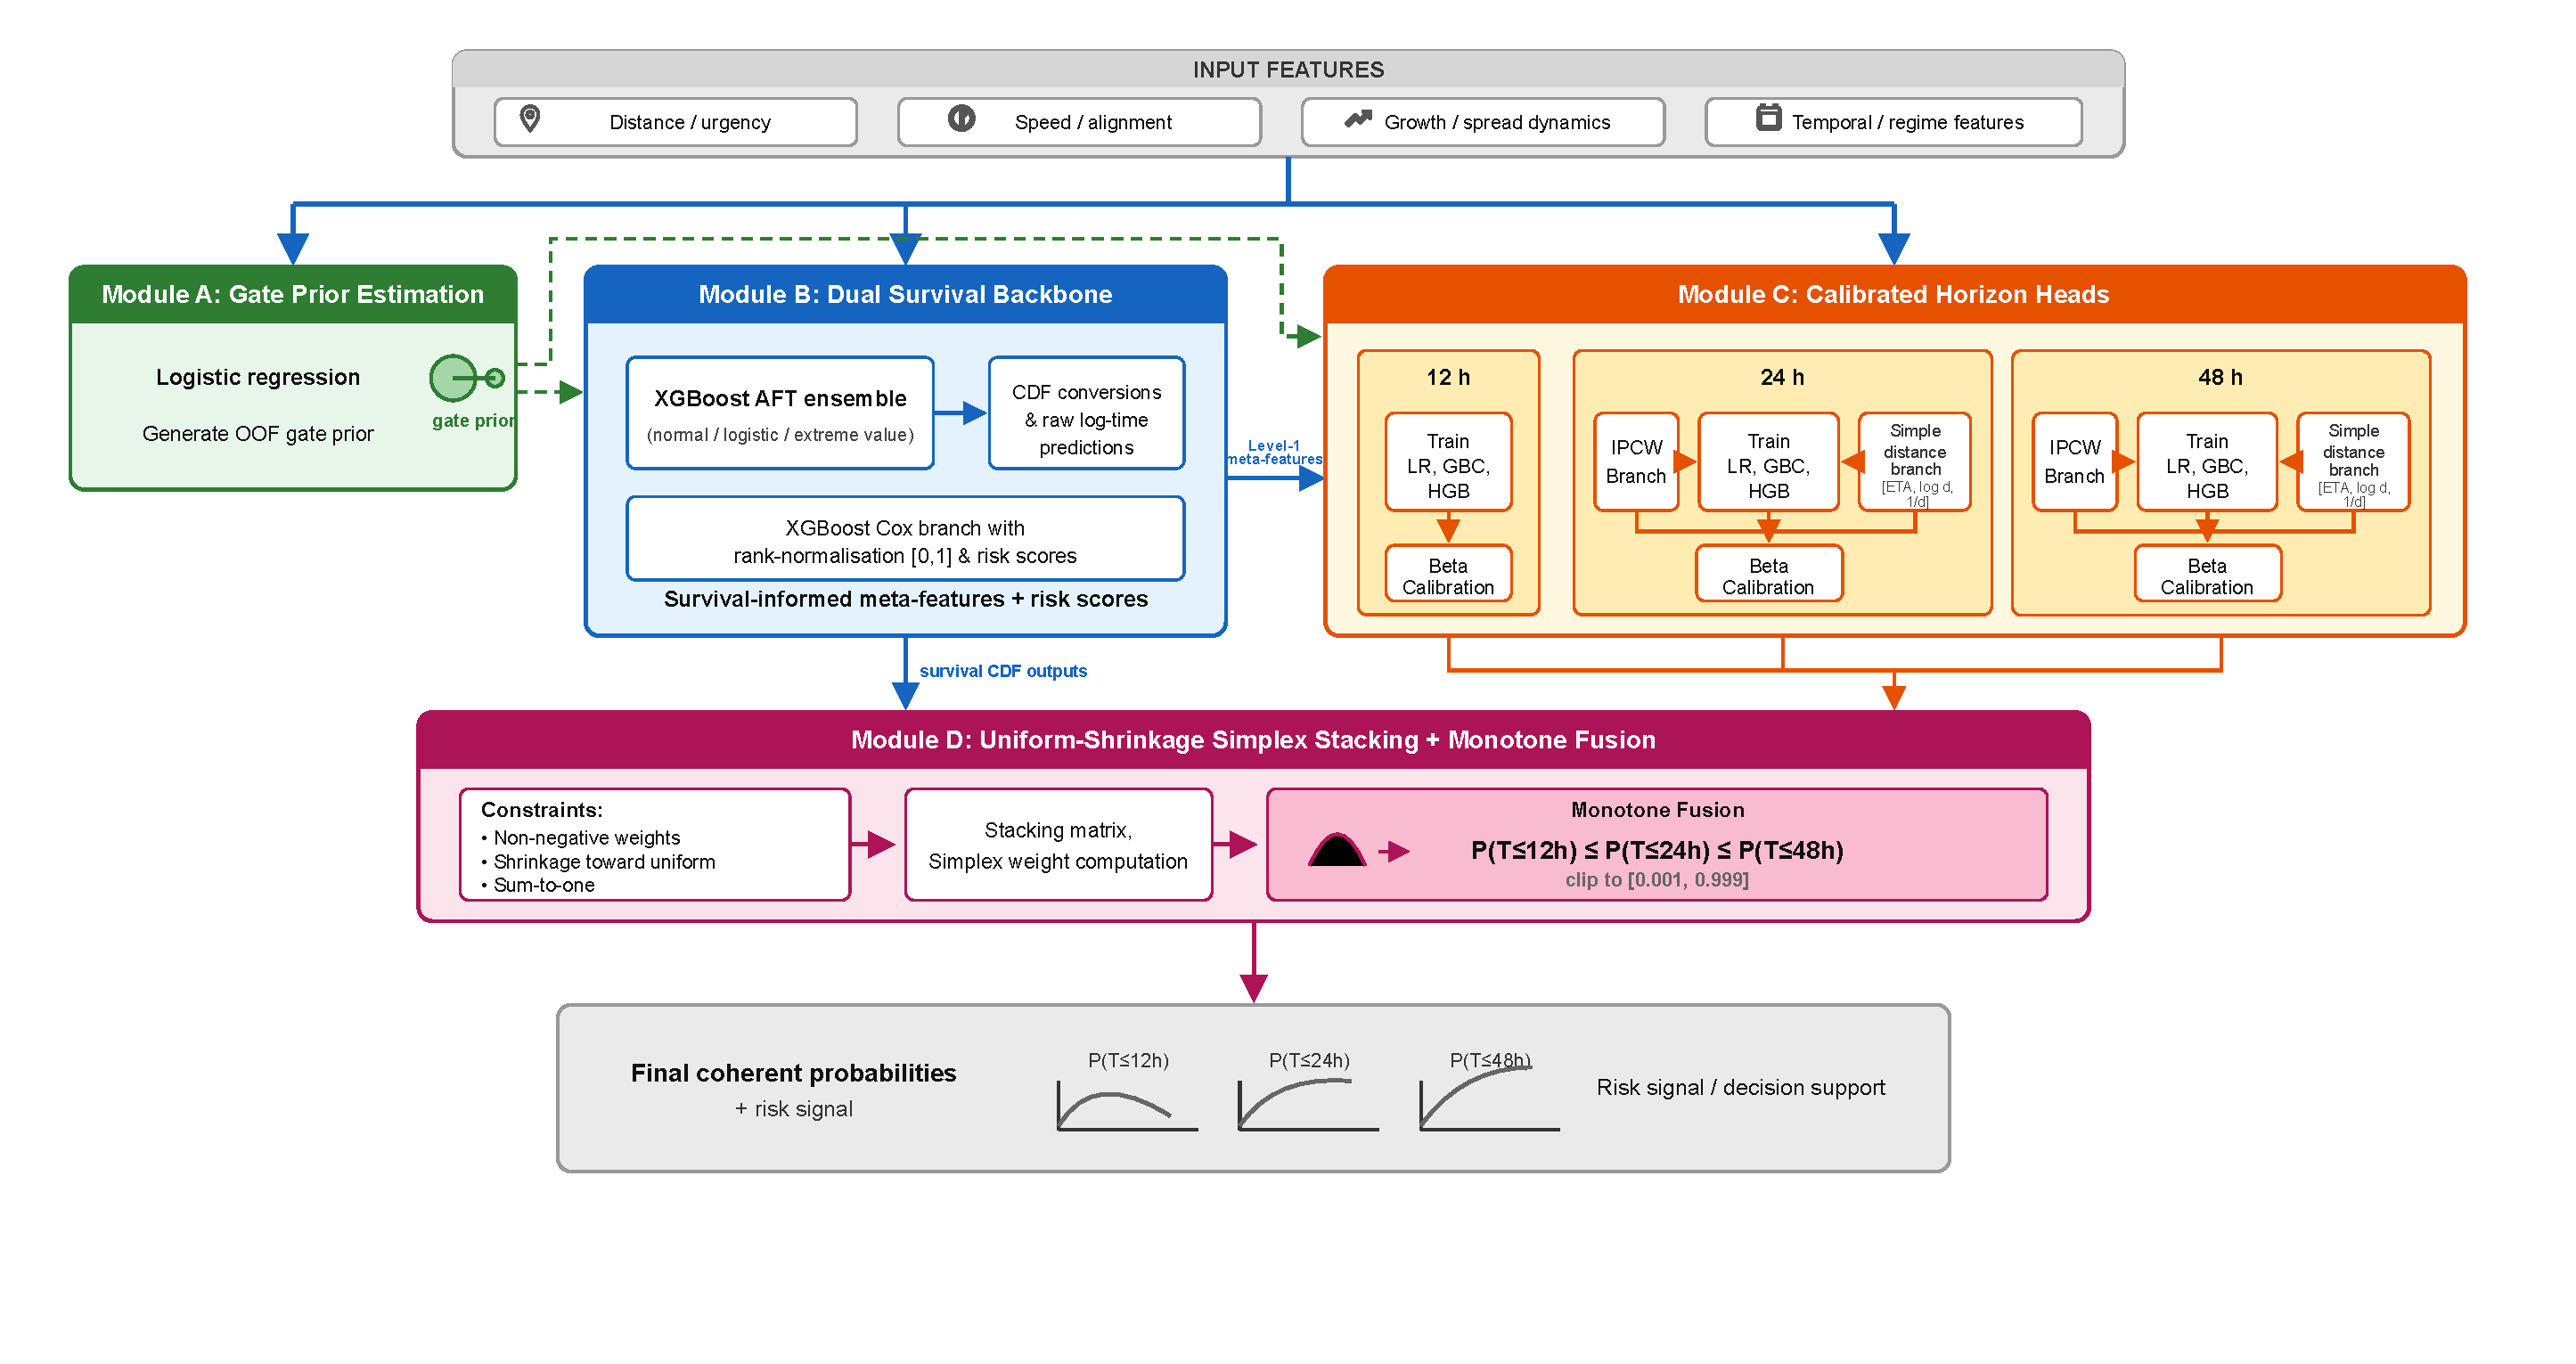
\includegraphics[width=\linewidth]{figures/main/Figure_2_framework_schematic.pdf}
\end{adjustwidth}
    \caption{Framework schematic. Module~A estimates a gate prior via logistic regression. Module~B comprises a dual survival backbone (XGBoost AFT and Cox proportional hazards). Module~C trains calibrated direct probability heads (logistic regression, gradient boosting, histogram gradient boosting with beta calibration) at each horizon. Module~D performs uniform-shrinkage simplex stacking followed by monotone-constrained fusion to produce final coherent probabilities $P(T \leq h)$ for $h \in \{12, 24, 48\}$.}\label{fig:framework}
\end{figure}

\subsubsection{Module A: Gate Prior Estimation}

As a first step, we fit a logistic regression to the full feature set with a binary event indicator as target.
The out-of-fold (OOF) predictions from this model serve as a \emph{gate prior}---a single soft score that summarises how likely each zone is to be reached by the fire---and are carried forward as an additional input to Modules~B and C.
In practice, this step distils the raw feature space into one stacking-level shrinkage signal, trimming redundancy before the heavier survival components process it.

\subsubsection{Module B: Dual Survival Backbone}

The backbone consists of two complementary survival branches:

\emph{XGBoost AFT ensemble.}
We fit three XGBoost~\cite{Chen2016} AFT models, each assuming a different error distribution (normal, logistic, extreme value) and using a different hyperparameter configuration.
For every observation the predicted log-survival time from each model is converted into a horizon-specific probability through the relevant distributional CDF.
These AFT-derived probabilities, together with the raw log-time predictions, constitute the survival-informed meta-features.

\emph{Cox proportional-hazards ranking branch.}
Three XGBoost Cox models with varying tree depth and learning rate settings are fit on the same features.
Their predicted risk scores supply a discrimination-oriented signal that complements the AFT branch's focus on probability estimation.
Before entering the stacking matrix, risk scores are rank-normalised to the $[0, 1]$ interval.

Both branches see only inner-fold data during training; OOF predictions are generated via cross-fitting, so no observation's meta-features are ever derived from a model that was trained on that same observation.

\emph{Design note on the Cox branch's role.}
An important architectural choice is that the Cox branch feeds only into the composite ranking signal used for discrimination reporting; it does \emph{not} enter the horizon-wise probability stacking matrix in Module~D.
As a result, toggling the Cox branch on or off can shift the concordance index but will leave Brier scores, ECE, and calibration slopes untouched.
We made this separation deliberately---the Cox branch is meant to sharpen ranking, not to adjust probability levels.

\subsubsection{Module C: Calibrated Horizon Heads}

At each horizon $h \in \{12, 24, 48\}$ we train three direct classifiers---logistic regression (LR), gradient boosting (GBC), and histogram gradient boosting (HGB)---targeting the censor-aware binary label $Y_h$.
Inputs to these classifiers include all Level~1 meta-features from Modules~A and~B plus the original engineered features.
After obtaining each classifier's OOF probability outputs, we apply three-parameter beta calibration~\cite{Kull2017} to sharpen probability reliability; calibration parameters are estimated on the inner-fold OOF set and then applied to outer-fold predictions.
A caveat: when the effective eligible sample within an inner fold is small (sometimes as few as $\sim$35 observations at certain horizons), three-parameter beta calibration may itself overfit; a two-parameter variant or isotonic regression could prove more robust and is worth exploring in follow-up work.

At the 24~h and 48~h horizons two supplementary branches may optionally be included:
(i)~an inverse-probability-of-censoring-weighted (IPCW) branch built on LightGBM classifiers, where each observation receives a weight $w_i = \delta_i / \hat{G}(T_i)$---$\delta_i$ being the event indicator and $\hat{G}(T_i)$ the Kaplan--Meier estimate of the censoring survival function at the observed time~\cite{Uno2011,Graf1999}; censored cases get zero weight and thus contribute nothing to the IPCW loss, which is the standard formulation; and
(ii)~a simple distance-based branch: a logistic regression on the $[\text{ETA}, \log d, 1/d]$ feature triple, acting as a physics-informed anchor.

\subsubsection{Module D: Uniform-Shrinkage Simplex Stacking and Monotone Fusion}

The horizon-specific probability estimates from Module~C, together with the survival CDF conversions from Module~B, are assembled into a single stacking matrix~\cite{Wolpert1992,VanderLaan2007}.
Fusion weights are obtained by minimising the Brier score~\cite{Brier1950} on the inner OOF set under non-negativity constraints, with a regularisation term that pulls the weight vector toward the uniform distribution (Equation~\eqref{eq:stacking}):
\begin{equation}
    \mathbf{w}^* = \arg\min_{\mathbf{w} \geq 0} \left[ \frac{1}{n} \sum_{i=1}^{n} \left( y_i - \mathbf{w}^\top \mathbf{s}_i \right)^2 + \lambda \left\| \mathbf{w} - \frac{1}{K}\mathbf{1} \right\|_2^2 \right],
    \label{eq:stacking}
\end{equation}
where $\mathbf{s}_i$ collects the stacked probability estimates for observation $i$, $K$ counts the base learners, and $\lambda = 1.0$ is a fixed regularisation strength (not tuned on data).
We set $\lambda = 1.0$ to impose moderate shrinkage: the data-driven Brier loss is typically $O(10^{-2})$ per observation, so a penalty of comparable magnitude discourages any single base learner from dominating while still allowing informative weight differentiation.
A sweep over $\lambda \in \{0.1, 0.5, 1.0, 2.0, 5.0\}$ confirmed that the headline metrics were insensitive to this choice (Supplementary Table~S2).
The problem is a convex quadratic program; we solved it with \texttt{scipy.optimize.minimize} (L-BFGS-B, bound constraints) and checked convergence in every fold.
Weights are then normalised to sum to one.

After stacking, a monotone-constrained fusion step forces $P(T \leq 12) \leq P(T \leq 24) \leq P(T \leq 48)$ by propagating the running maximum across horizons and clipping to $[0.001, 0.999]$.

\subsection{Validation Design}\label{sec:validation}

To guard against information leakage and to obtain performance estimates we can trust, we employed a nested cross-validation scheme following standard guidance for prediction model studies~\cite{Wolff2019,Steyerberg2019}.

\emph{Outer loop} (5 folds, stratified by event-time strata). Every metric we report comes from the out-of-fold predictions of this loop.
We stratified folds using discretised event-time quintiles for events and a single catch-all stratum for censored cases, giving each fold a representative event-rate mix.
One important caveat: the dataset lacks a verified wildfire-incident identifier. If multiple fire--zone pairs originate from the same wildfire, they may land in both the training and validation folds of a given outer split---a potential source of optimistic bias, since observations from the same incident share fire-trajectory and terrain characteristics.
We could not perform a true incident-grouped split, so we ran two auxiliary checks instead. A proxy incident-grouped analysis used hierarchical clustering on the 12 most discriminative covariates to carve out 43 pseudo-incident groups; a lean AFT model was then evaluated under both standard stratified and GroupKFold splitting to gauge how much the C-index dropped (Supplementary Table~S8, Figure~S2).
Separately, a leave-one-month-out temporal blocked analysis with the same lean AFT model provided a conservative temporal robustness check (Supplementary Figure~S3).
Both auxiliary analyses were intended as \emph{relative-bias probes} on the validation scheme---not as absolute performance benchmarks for the full multi-module prototype, which would be starved of data under such restrictive partitions.

\emph{Inner loop} (5 folds nested inside each outer training set). This loop has a dual job: producing the meta-features consumed by downstream modules (Level~1: gate prior, AFT log-time predictions, Cox risk scores; Level~2: direct heads, IPCW, simple branch) and fitting the stacking fusion weights.
The key constraint is that an observation's fusion weight is never estimated from meta-features generated by a model that was trained on that observation.
A 5$\times$5 fold layout was selected as a reasonable bias--variance compromise at $n = 221$; using fewer folds would widen variance, while using more would leave the inner training sets too thin~\cite{Steyerberg2019}.

For 95\% bootstrap CIs we resampled the outer-fold OOF predictions 1000 times (stratified) and took the 2.5th and 97.5th percentiles. At the metric magnitudes we observe, 1000 resamples are more than adequate for stable CI bounds~\cite{Efron1993}.

\subsection{Baselines and Ablations}\label{sec:baselines}

Four baselines of increasing strength were pitted against the full framework:
(i)~\emph{ETA-only}---logistic regression predicting each horizon target from the estimated time-of-arrival feature alone, serving as the simplest physics-informed reference;
(ii)~\emph{AFT-only}---the three-AFT ensemble with CDF-derived horizon probabilities and monotone fusion, but without any of the direct heads, Cox, IPCW, or simple branches;
(iii)~\emph{Per-horizon XGBoost}---a stand-alone XGBoost classifier fit separately at each horizon on all 34 features using the censor-aware eligible subset, representing a strong single-model ML comparator that carries no survival structure;
(iv)~\emph{Random Survival Forest} (RSF)~\cite{Ishwaran2008}---500 trees with log-rank splitting, CDF-derived probabilities, and monotone fusion. As a nonparametric survival method in its own right, RSF provides a head-to-head survival-side competitor.

The ablation study followed two complementary tracks.
The \emph{layered build-up} started from the bare AFT backbone and bolted on module groups one at a time (AFT~$\to$ AFT~+~Direct~$\to$ AFT~+~Direct~+~Cox, or alternatively AFT~+~Direct~+~Gate, culminating in the Full model). Note that these are parallel branches rather than a single chain: AFT~+~Direct~+~Cox and AFT~+~Direct~+~Gate each extend the AFT~+~Direct base in a different direction.
The \emph{component removal} track began with the full model and disabled one module at a time (w/o~Gate, w/o~Cox, w/o~IPCW, w/o~Simple Distance, w/o~Direct Heads, Thin~Features~only), checking whether each omission made things worse.

Statistical significance was evaluated with a paired delta-metric bootstrap (1000 resamples). For each comparison we tested the directional null $\Delta\text{C-index}_{\text{full} - \text{ablated}} = 0$ and $\Delta\text{IBS}_{\text{full} - \text{ablated}} = 0$, computing one-sided $p$-values as the fraction of resamples in which the full model failed to beat the reduced variant. This one-sided setup matches our prior expectation that adding modules should at worst be neutral~\cite{Collins2024}.
We caution that with $n = 221$ and 69 events, effect sizes and bootstrap CIs are more informative than raw $p$-values; the latter should be read as directional cues, not formal hypothesis tests.
Two-sided $p$-values are available in Supplementary Table~S3.

\subsection{Practical Lean Variants and Stability Analysis}\label{sec:lean_variants}

At an EPV ratio of about 2.0, the full architecture is arguably carrying more machinery than the data can support---its many stacking layers may end up injecting more estimation noise than the signal can absorb.
To see how much complexity can be stripped away without losing performance, we evaluated three leaner variants under the same nested CV protocol:
(i)~\emph{AFT~+~Cox}---the AFT backbone paired only with the Cox ranking branch, preserving censor-aware probabilities while adding a discrimination boost;
(ii)~\emph{AFT~+~Cox~+~Simple}---same as above, but with the simple distance-based logistic head at 24~h and 48~h appended as a physics-grounded anchor;
(iii)~\emph{AFT~+~Simple}---AFT backbone plus simple distance head, with Cox dropped entirely.
Thin-feature variants (26 engineered features only, no original dataset columns) were run as a supplementary check but offered no clear stability gain, so they are left out of the main text.

To test whether model rankings depended on the particular random seed governing fold assignment, we re-ran every core model---Full, AFT~+~Cox, AFT~+~Cox~+~Simple, Per-horizon XGBoost, and RSF---under five seeds (42, 123, 314, 2024, 7777).
Mean and standard deviation of C-index and IBS across these seeds serve as our stability diagnostic.
This seed-based check sits alongside the proxy incident-grouped analysis in Section~\ref{sec:validation}; the latter could only be run for a lean AFT model because verified incident identifiers are absent from the dataset.

\subsection{Evaluation Metrics}\label{sec:metrics}

\paragraph{Discrimination.}
We computed two concordance measures.
A pairwise concordance index proxy~\cite{Harrell1996} (Harrell-style pairwise implementation) was obtained by comparing all concordant and discordant pairs within the eligible observations.
We also computed Uno's IPCW C-statistic~\cite{Uno2011}, which adjusts for censoring; both values are reported side by side, with Uno's C treated as the preferred measure for censored data.

\paragraph{Calibration and probability error.}
For every horizon, Brier scores~\cite{Brier1950} were computed on the censor-aware eligible subsets.
Expected calibration error (ECE) and maximum calibration error (MCE) were extracted from decile-binned reliability diagrams~\cite{NiculescuMizil2005}.
We additionally fit a logistic recalibration model---predicting observed outcomes from predicted probabilities---to obtain a calibration slope and intercept~\cite{VanCalster2019}. A slope hovering around 1.0 with an intercept near 0.0 signals well-calibrated predictions; slopes below 1 reveal overconfidence, and slopes above 1 point to underconfidence.

\paragraph{Summary error measure.}
As an overall error summary, we took the arithmetic mean of the three horizon-specific Brier scores (12, 24, 48~h) and call it the IBS proxy.
Strictly speaking, this is not a true continuous-time integrated Brier score~\cite{Graf1999}---a distinction we want to flag explicitly.

\paragraph{Monotonicity.}
We counted how many observations violated $P(T \leq h_1) \leq P(T \leq h_2)$ at each pair of adjacent horizons.

\paragraph{Decision utility and decision curve analysis.}
To gauge the framework's usefulness for threshold-based evacuation triggers, we computed sensitivity, specificity, PPV, NPV, and F1 at several probability cut-offs (0.1, 0.2, 0.3, 0.5, 0.7) per horizon.
On top of this, we ran a decision curve analysis (DCA)~\cite{Vickers2006} sweeping $p_t$ over $[0.01, 0.99]$ and benchmarking the model against two na\"ive reference strategies: ``evacuate every zone'' and ``evacuate none.''
Net benefit at threshold $p_t$ was computed as $\text{NB} = \text{TPR} \cdot \pi - \text{FPR} \cdot (1 - \pi) \cdot w$, where $\pi$ is the event prevalence and $w = p_t / (1 - p_t)$.

\subsection{Sensitivity Analysis: Joint Post-Fusion Recalibration}\label{sec:recal}

As a sensitivity check, we applied a joint post-fusion recalibration step to see whether horizon-specific calibration could be tightened after stacking and monotone fusion.
Specifically, we divided the 12~h predicted logits by a temperature parameter $T$, chosen by grid search ($T \in [0.5, 3.0]$, step~0.1) to minimise the 12~h Brier score on OOF predictions, then re-applied the monotone fusion step so that the correction would propagate to 24~h and 48~h.
A legacy variant that temperature-scaled only 12~h (without re-optimising the longer horizons) was also included for comparison.
Neither variant influenced primary model selection or altered the training/evaluation pipeline; they are reported purely to characterise the cross-horizon calibration trade-off and to inform potential deployment choices.

\subsection{Software and Reproducibility}\label{sec:software}

The entire analysis was implemented in Python~3.10, relying on scikit-learn~1.3, XGBoost~2.0, LightGBM~4.1, and lifelines~0.28.
A fixed random seed of 42 was used for the primary run; on top of that, we conducted a five-seed stability analysis (seeds 42, 123, 314, 2024, 7777) to check whether model rankings were sensitive to how folds happened to be assigned.
Both outer and inner cross-validation used $K_{\text{outer}} = K_{\text{inner}} = 5$ stratified folds.
All code and curated supplementary files are available at \url{https://github.com/eee-afkk/wids2026-wildfire-survival}.
Generative AI assistance (Claude, Anthropic) was used solely for English language editing and stylistic polishing of author-written text; it was not involved in study design, data processing, statistical analysis, figure generation, or interpretation of results.

\section{Results}\label{sec:results}

\subsection{Cohort Characteristics}\label{sec:cohort}

Our cohort consisted of 221 wildfire--zone encounters; 69 of them (31.2\%) ended in an observed event.
Table~\ref{tab:horizons} breaks down the eligible sample sizes and positive rates by prediction horizon.
At 12~h the positive rate was lowest (22.8\%), reflecting the narrow time window; by 48~h it climbed to 39.8\%.
The 72~h horizon was degenerate---every one of the 69 eligible observations experienced the event---and was dropped from further analysis.

\subsection{Primary Model Performance}\label{sec:primary}

Everything reported below refers to the pre-recalibration model, scored on nested OOF predictions.
Table~\ref{tab:primary} collects the headline metrics together with 95\% bootstrap CIs.

\begin{table}[!ht]
\caption{Primary model performance (pre-recalibration, nested OOF evaluation). CI = 95\% bootstrap confidence interval (1000 resamples).}\label{tab:primary}
\begin{tabular}{lcc}
\toprule
\textbf{Metric} & \textbf{Estimate} & \textbf{95\% CI} \\
\midrule
Pairwise concordance index proxy & 0.940 & [0.927, 0.955] \\
Uno's IPCW C-index               & 0.941 & [0.924, 0.959] \\
Mean Brier (IBS proxy)           & 0.041 & [0.025, 0.058] \\
Brier @ 12~h                     & 0.060 & [0.038, 0.086] \\
Brier @ 24~h                     & 0.035 & [0.017, 0.058] \\
Brier @ 48~h                     & 0.027 & [0.009, 0.050] \\
\bottomrule
\end{tabular}
\end{table}

A concordance index of 0.940 (Uno's IPCW C-index: 0.941) means the model put threat times in the right order for more than 94\% of all comparable wildfire--zone pairs.
Brier scores were low at every horizon, dropping from 0.060 at 12~h to 0.027 at 48~h.

\subsection{Calibration and Reliability}\label{sec:calibration}

Horizon-by-horizon calibration numbers are laid out in Table~\ref{tab:calibration}; Figure~\ref{fig:reliability} shows the corresponding reliability diagrams.

\begin{table}[!ht]
\caption{Calibration summary by prediction horizon (pre-recalibration).}\label{tab:calibration}
\begin{tabular}{lcccccc}
\toprule
\textbf{Horizon} & $n$ & \textbf{Brier} & \textbf{ECE} & \textbf{MCE} & \textbf{Cal.\ Slope} & \textbf{Cal.\ Intercept} \\
\midrule
12~h & 215 & 0.060 & 0.057 & 0.556 & 0.805 & 0.245 \\
24~h & 196 & 0.035 & 0.014 & 0.651 & 0.998 & $-$0.061 \\
48~h & 166 & 0.027 & 0.031 & 0.777 & 1.075 & $-$0.272 \\
\bottomrule
\end{tabular}
\end{table}

\begin{figure}[!ht]
\begin{adjustwidth}{-\extralength}{0cm}
    \centering
    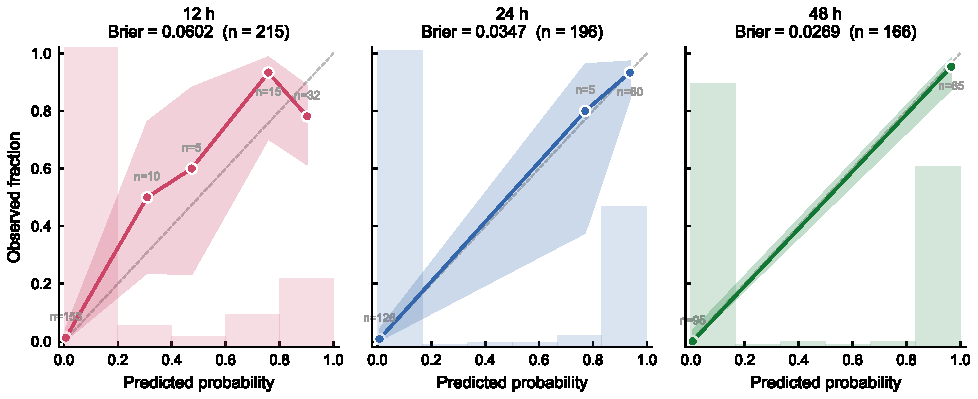
\includegraphics[width=\linewidth]{figures/main/Figure_3_reliability_diagrams.pdf}
\end{adjustwidth}
    \caption{Reliability diagrams for 12, 24, and 48~h horizons (pre-recalibration, nested OOF). Shaded bands represent Wilson confidence intervals. Histograms show predicted probability distributions. The dashed diagonal indicates perfect calibration.}\label{fig:reliability}
\end{figure}

The 24~h horizon was clearly the best calibrated of the three (slope~=~0.998; ECE~=~0.014)---its reliability curve tracked the diagonal almost exactly.
At 48~h, calibration was acceptable though leaning slightly underconfident (slope~=~1.075; ECE~=~0.031).
Calibrating the 12~h horizon turned out to be the hardest task: a slope of 0.805 flagged meaningful overconfidence, and the ECE of 0.057 underscored how challenging short-horizon predictions are in this setting.
Figure~\ref{fig:calsummary} visualises how Brier score, ECE, and calibration slope change with horizon length.
MCE rose from 0.556 (12~h) to 0.777 (48~h)---not because average calibration deteriorated, but because sparsely populated high-probability bins inflate single-observation deviations.
The calibration intercept switched sign, moving from +0.245 at 12~h (systematic under-prediction of risk) to $-$0.272 at 48~h (over-prediction), a pattern the monotone fusion step likely accentuated by pushing 24~h probabilities upward into the 48~h estimates.
In operational terms, the 24~h output is the one to trust for absolute-threshold evacuation decisions; the 12~h output should be handled cautiously when used with fixed probability triggers (post-fusion recalibration is examined in Section~\ref{sec:recal_results}).

\begin{figure}[!ht]
\begin{adjustwidth}{-\extralength}{0cm}
    \centering
    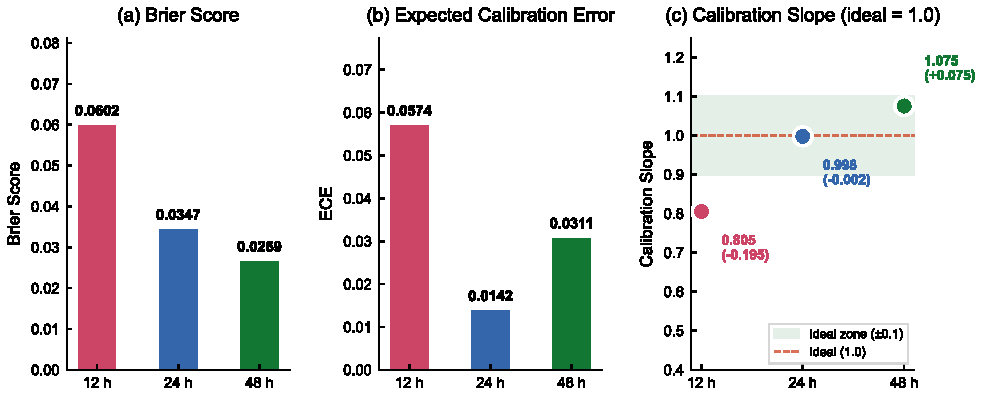
\includegraphics[width=\linewidth]{figures/main/Figure_4_calibration_summary.pdf}
\end{adjustwidth}
    \caption{Calibration summary: (a)~Brier score, (b)~expected calibration error (ECE), and (c)~calibration slope by horizon. The dashed line in~(c) indicates the ideal slope of 1.0.}\label{fig:calsummary}
\end{figure}

\subsection{Baseline Comparison}\label{sec:baseline_results}

Table~\ref{tab:baseline} and Figure~\ref{fig:baseline} present the baseline comparison.

\begin{table}[!ht]
\caption{Core model comparison (all models evaluated under the same nested OOF protocol, seed~=~42). IBS = mean Brier score across 12/24/48~h horizons. Uno-C = Uno's IPCW C-index. Models are grouped by role: physics-informed baseline, survival-centred lean variants, external comparators, and the full prototype.}\label{tab:baseline}
\begin{adjustwidth}{-0.5\extralength}{-0.5\extralength}
\centering
\footnotesize
\begin{tabular}{llcccccc}
\toprule
\textbf{Role} & \textbf{Model} & \textbf{C-index} & \textbf{Uno-C} & \textbf{IBS} & \textbf{Brier@12\,h} & \textbf{Brier@24\,h} & \textbf{Brier@48\,h} \\
\midrule
Baseline          & ETA-only (LR)            & 0.908 & 0.910 & 0.045 & 0.070 & 0.038 & 0.028 \\
\midrule
\multirow{3}{*}{\parbox{1.6cm}{Lean\\variants}} 
                  & AFT Only                 & 0.938 & 0.940 & 0.039 & 0.055 & 0.035 & 0.027 \\
                  & AFT + Cox                & 0.939 & 0.940 & 0.039 & 0.055 & 0.035 & 0.027 \\
                  & AFT + Cox + Simple       & 0.941 & 0.942 & 0.038 & 0.055 & 0.035 & 0.025 \\
\midrule
\multirow{2}{*}{\parbox{1.6cm}{External\\comparators}}
                  & Per-horizon XGBoost      & 0.942 & 0.943 & 0.040 & 0.056 & 0.037 & 0.026 \\
                  & Random Survival Forest   & 0.940 & 0.941 & 0.032 & 0.051 & 0.028 & 0.018 \\
\midrule
Prototype         & Full Model               & 0.940 & 0.941 & 0.041 & 0.060 & 0.035 & 0.027 \\
\bottomrule
\end{tabular}
\end{adjustwidth}
\end{table}

\begin{figure}[!ht]
\begin{adjustwidth}{-\extralength}{0cm}
    \centering
    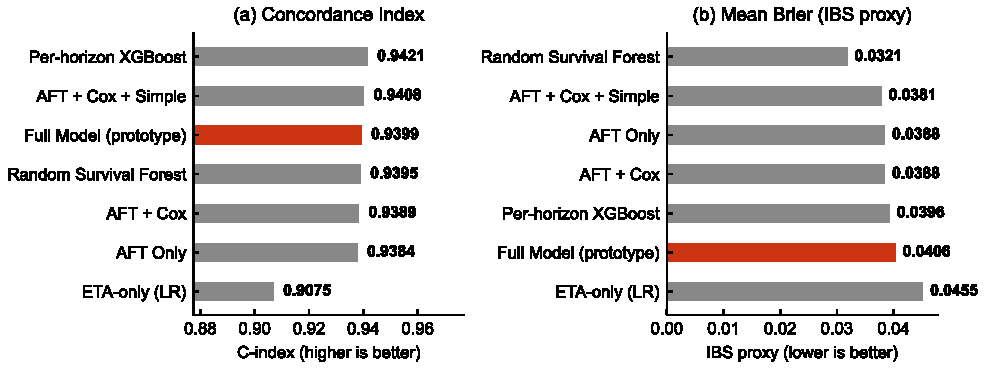
\includegraphics[width=\linewidth]{figures/main/Figure_5_baseline_comparison.pdf}
\end{adjustwidth}
    \caption{Baseline comparison: (a)~pairwise concordance index proxy and (b)~integrated Brier score proxy. Higher C-index and lower IBS are better.}\label{fig:baseline}
\end{figure}

The full prototype beat the physics-informed ETA-only baseline convincingly ($\Delta$C-index = +0.032) but could not consistently outdo the stronger competitors.
At a sample size of 221, what the framework offers is structural---coherent, censor-aware probability sequences---rather than dominance on every single metric.
Table~\ref{tab:baseline} groups the models into three functional tiers.

Looking at the \emph{lean AFT-centred variants}, AFT~+~Cox reached a C-index of 0.939, close to the full model.
AFT~+~Cox~+~Simple posted a lower IBS (0.038 vs.\ 0.041), hinting that the simple distance branch helps anchor the probability estimates.
By construction, AFT~Only and AFT~+~Cox produced identical Brier scores and calibration numbers---they differ only in C-index, because the Cox branch touches only the ranking signal.

Among the \emph{external comparators}, per-horizon XGBoost scored the highest C-index (0.942) and a comparable IBS (0.040), demonstrating that a well-tuned single-model strategy can rival the full framework when the dataset is this small.
The Random Survival Forest (C-index: 0.940, IBS: 0.032) turned in the lowest probability error of any model we tested.

In the paired bootstrap analysis, the gap between the full model and AFT-only was $\Delta$C-index = +0.002 [$-$0.002, +0.004] ($p = 0.170$), and $\Delta$IBS = $-$0.002 ($p = 0.805$)---neither significant.
The RSF comparison merits special attention: RSF is itself censor-aware and inherently produces monotone probabilities.
At this data scale, RSF's lower IBS and tighter seed-to-seed stability point to a single integrated survival model absorbing the available signal more efficiently than the full stacked architecture does. The modular design of our framework remains a research-oriented advantage, but one that awaits confirmation on larger datasets.

\subsection{Ablation Study}\label{sec:ablation_results}

Figure~\ref{fig:ablation} presents the ablation forest plot, and Table~\ref{tab:ablation} reports detailed results.

\begin{figure}[!ht]
\begin{adjustwidth}{-\extralength}{0cm}
    \centering
    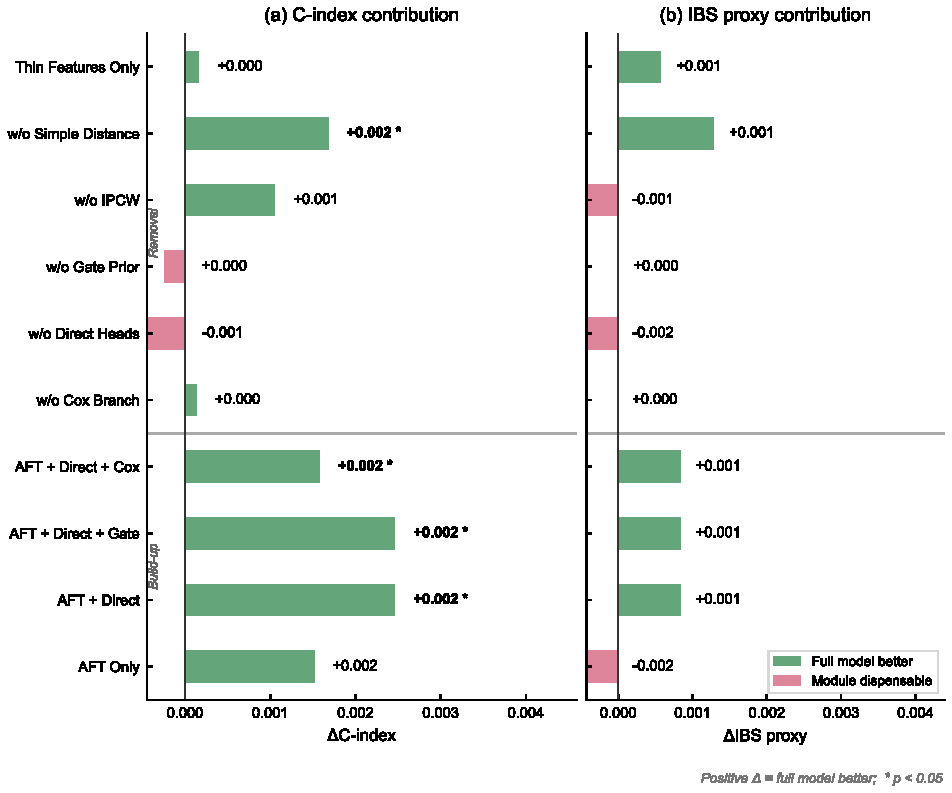
\includegraphics[width=\linewidth]{figures/main/Figure_6_ablation_contribution_summary.pdf}
\end{adjustwidth}
    \caption{Ablation forest plot showing the contribution of each configuration relative to the full model ($\Delta$C-index and $\Delta$IBS). Positive values indicate that the full model outperformed the ablated variant. Asterisks denote significance at $p < 0.05$ from paired bootstrap.}\label{fig:ablation}
\end{figure}

\begin{table}[!ht]
\caption{Ablation study: paired delta-metric bootstrap results (1000 resamples). $\Delta > 0$ indicates full model superiority. CI = 95\% bootstrap confidence interval. $p$ = one-sided. Significance: * $p < 0.05$. $^\ddagger$For the w/o~Cox~Branch configuration, $\Delta\text{IBS} = 0.000$ by architectural design: the Cox branch is isolated from the probability stacking matrix in Module~D and therefore cannot alter Brier scores or ECE. The significant one-sided $p$ reflects that the full model matched or exceeded the ablated variant in every bootstrap resample, consistent with non-negativity of the constraint.}\label{tab:ablation}
\small
\begin{tabular}{lcccc}
\toprule
\textbf{Configuration} & \textbf{$\Delta$C-index [95\% CI]} & \textbf{$p$} & \textbf{$\Delta$IBS [95\% CI]} & \textbf{$p$} \\
\midrule
AFT Only           & +0.002 [$-$0.002, +0.004] & 0.340 & $-$0.002 [$-$0.006, +0.003] & 0.390 \\
AFT + Direct       & +0.002 [+0.000, +0.005]* & 0.024 & +0.001 [$-$0.002, +0.004] & 0.588 \\
AFT + Direct + Cox & +0.002 [$-$0.000, +0.003] & 0.096 & +0.001 [$-$0.002, +0.004] & 0.588 \\
AFT + Direct + Gate & +0.002 [+0.000, +0.005]* & 0.024 & +0.001 [$-$0.002, +0.004] & 0.588 \\
w/o Gate Prior     & $-$0.000 [$-$0.001, +0.000] & 0.064 & +0.000 [$-$0.000, +0.000] & 0.524 \\
w/o Cox Branch     & +0.000 [$-$0.002, +0.002] & 0.892 & +0.000 [+0.000, +0.000]$^\ddagger$ & $<$0.001 \\
w/o IPCW           & +0.001 [$-$0.000, +0.002] & 0.110 & $-$0.001 [$-$0.002, +0.001] & 0.400 \\
w/o Simple Dist.   & +0.002 [+0.000, +0.004]* & 0.050 & +0.001 [$-$0.001, +0.004] & 0.312 \\
w/o Direct Heads   & $-$0.001 [$-$0.003, +0.001] & 0.422 & $-$0.002 [$-$0.005, +0.001] & 0.126 \\
Thin Features      & +0.000 [$-$0.006, +0.006] & 0.964 & +0.001 [$-$0.005, +0.006] & 0.834 \\
\bottomrule
\end{tabular}
\end{table}

On internal ablation metrics the full framework held a slight discrimination edge, although external baselines like per-horizon XGBoost and RSF matched or beat it on aggregate (see Section~\ref{sec:baseline_results}).
The individual modules contributed unevenly.
Dropping the \emph{Cox branch} left $\Delta$C-index at +0.000 ($p = 0.892$) and $\Delta$IBS at exactly zero ($p < 0.001$)---as expected, since the Cox branch feeds only the ranking signal and is architecturally excluded from the probability stacking matrix; the non-zero $p$-value reflects that the full model matched or exceeded the ablated variant in every bootstrap resample.
The \emph{simple distance branch} mattered for both discrimination and probability error ($\Delta$C-index = +0.002, $p = 0.050$; $\Delta$IBS = +0.001, $p = 0.312$).
The \emph{gate prior} and \emph{IPCW} modules registered only marginal standalone effects; their contributions may be masked by the other components or may surface with more data.

In the build-up arm, AFT~+~Direct fell significantly short of the full model ($\Delta$C-index = +0.002, $p = 0.024$), whereas the AFT-only gap was comparable in magnitude but not significant ($\Delta = +0.002$, $p = 0.340$).
The implication is that direct heads, when bolted on alone, add estimation noise that the remaining modules (Cox, gate prior, IPCW, simple distance) must counteract. Stripping direct heads out of the full model even improved IBS slightly ($\Delta = -0.002$, $p = 0.126$), which fits the same picture.
Once the Cox branch was added to AFT~+~Direct the C-index deficit narrowed ($p = 0.096$), consistent with its discrimination-boosting role.

\subsection{Bootstrap Confidence Intervals}\label{sec:bootstrap}

Figure~\ref{fig:bootstrap} plots the bootstrap distributions for the primary metrics.
The C-index distribution clustered tightly around a median of 0.940 (95\% CI: [0.927,~0.955]), and the Uno's IPCW C-index (0.941, [0.924,~0.959]) corroborated steady censoring-adjusted discrimination.
The IBS proxy landed at 0.041 ([0.025,~0.058]); horizon-level Brier distributions confirmed low probability error, with CI widths reflecting what one expects at $n = 221$.
All these distributions pertain to pre-recalibration predictions.

\begin{figure}[!ht]
\begin{adjustwidth}{-\extralength}{0cm}
    \centering
    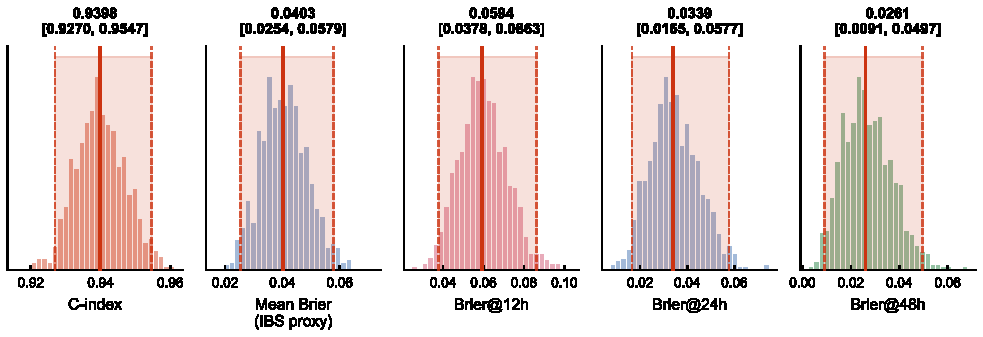
\includegraphics[width=\linewidth]{figures/main/Figure_7_bootstrap_confidence_intervals.pdf}
\end{adjustwidth}
    \caption{Bootstrap confidence interval distributions (1000 stratified resamples, pre-recalibration) for primary performance metrics. Solid red lines indicate medians; dashed red lines indicate the 2.5th and 97.5th percentiles defining 95\% CIs. Shaded bands span the CI region.}\label{fig:bootstrap}
\end{figure}

\subsection{Risk Stratification and Monotonicity}\label{sec:stratification}

Once monotone-constrained fusion (Module~D) was applied, not a single violation of $P(T \leq h_1) \leq P(T \leq h_2)$ remained across all 221 observations---which is guaranteed by construction.
The more revealing diagnostic is what happened \emph{before} fusion: the 12~h~$\to$~24~h transition produced zero violations, but at the 24~h~$\to$~48~h boundary 55 out of 221 observations (24.9\%) had their probabilities out of order, with a mean absolute correction of 0.002 (maximum: 0.115).
Had we omitted the monotone step, about one in four observations would have received logically contradictory probability sequences at the 24--48~h transition---evidence that the enforcement module does genuine corrective work and is not merely cosmetic.
Scatter plots documenting this are in Figure~S1.

When we split the 24~h predictions into terciles, the resulting risk groups were strikingly well separated (Table~\ref{tab:stratification}; Figure~\ref{fig:distributions}).
The low-risk tercile ($n = 65$) saw zero events within 24~h (0.0\%; 95\% Wilson CI: 0.0--5.6\%); the medium-risk tercile ($n = 66$) recorded a 4.5\% event rate (CI: 1.6--12.5\%); and the high-risk tercile ($n = 65$) saw events in 92.3\% of cases (CI: 83.2--96.7\%).
We note that these cutpoints were derived from the OOF predictions and are therefore data-dependent; we have not formally tested how stable they are across repeated cross-validation runs.

\begin{table}[!ht]
\caption{Risk stratification by 24~h predicted probability terciles. Event rates and 95\% Wilson confidence intervals are computed on the censor-aware eligible subset ($n = 196$).}\label{tab:stratification}
\begin{tabular}{lccc}
\toprule
\textbf{Risk Tercile} & \textbf{$n$} & \textbf{Observed Event Rate (\%)} & \textbf{95\% Wilson CI} \\
\midrule
Low    & 65 & 0.0  & [0.0, 5.6] \\
Medium & 66 & 4.5  & [1.6, 12.5] \\
High   & 65 & 92.3 & [83.2, 96.7] \\
\bottomrule
\end{tabular}
\end{table}

\begin{figure}[!ht]
\begin{adjustwidth}{-\extralength}{0cm}
    \centering
    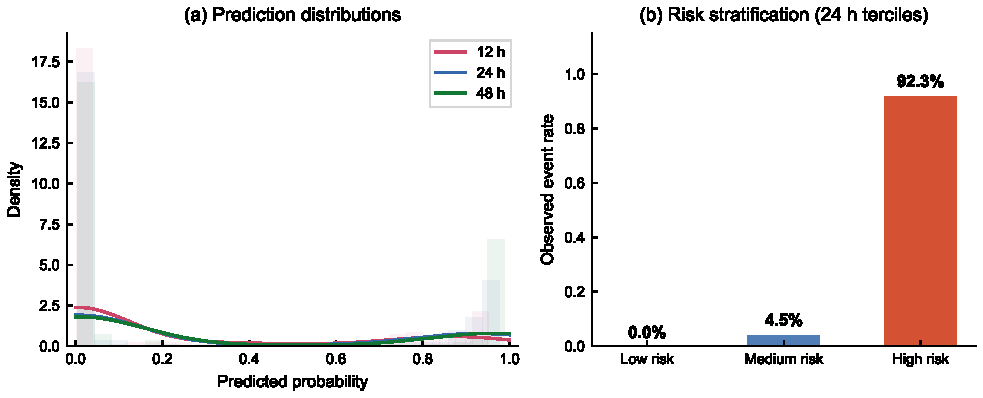
\includegraphics[width=\linewidth]{figures/main/Figure_8_prediction_distributions_and_risk_stratification.pdf}
\end{adjustwidth}
    \caption{(a)~Predicted probability distributions across the three horizons. The bimodal pattern reflects the clear separation between low- and high-threat cases under monotone-constrained fusion, consistent with the strong risk stratification observed in the data. (b)~Risk stratification by 24~h predicted probability terciles, with observed event rates of 0.0\% (low), 4.5\% (medium), and 92.3\% (high risk).}\label{fig:distributions}
\end{figure}

\subsection{Practical Lean Variants and Model Simplification}\label{sec:lean_results}

The lean AFT-centred variants sit alongside the external comparators and the full prototype in Table~\ref{tab:baseline}.
Paired bootstrap tests found no significant gap for either lean variant relative to the full model: AFT~+~Cox vs.\ Full ($\Delta$C-index = +0.001, $p = 0.260$; $\Delta$IBS = $-$0.002, $p = 0.805$) and AFT~+~Cox~+~Simple vs.\ Full ($\Delta$C-index = $-$0.001, $p = 0.762$; $\Delta$IBS = $-$0.002, $p = 0.869$). The latter actually posted a numerically lower IBS (0.038 vs.\ 0.041).

What this tells us is that the extra modules---direct heads, gate prior, IPCW---do not earn a statistically detectable payoff at the present sample size.
The Cox branch's contribution was limited to discrimination (C-index 0.939 vs.\ 0.938 for AFT~Only; probability metrics identical).
Meanwhile, the simple distance branch reduced probability error without touching discrimination (IBS = 0.038 vs.\ 0.039 for AFT~+~Cox).

\subsection{Multi-Seed Stability Analysis}\label{sec:stability}

Table~\ref{tab:stability} summarises the multi-seed stability results across five random seeds.

\begin{table}[!ht]
\caption{Multi-seed stability analysis (five seeds: 42, 123, 314, 2024, 7777). Mean and standard deviation of C-index and IBS proxy across seeds.}\label{tab:stability}
\begin{tabular}{lcc}
\toprule
\textbf{Model} & \textbf{C-index (mean $\pm$ SD)} & \textbf{IBS (mean $\pm$ SD)} \\
\midrule
Random Survival Forest & 0.941 $\pm$ 0.001 & 0.032 $\pm$ 0.000 \\
Per-horizon XGBoost    & 0.940 $\pm$ 0.001 & 0.039 $\pm$ 0.001 \\
AFT + Cox + Simple     & 0.939 $\pm$ 0.003 & 0.040 $\pm$ 0.001 \\
Full Model (prototype) & 0.938 $\pm$ 0.003 & 0.041 $\pm$ 0.002 \\
AFT + Cox              & 0.938 $\pm$ 0.003 & 0.040 $\pm$ 0.002 \\
\bottomrule
\end{tabular}
\end{table}

RSF was the most stable model by a clear margin (C-index SD = 0.001; IBS SD $<$ 0.001), with per-horizon XGBoost close behind (C-index SD = 0.001; IBS SD = 0.001).
The full model and its lean AFT cousins fluctuated more noticeably from seed to seed (C-index SD = 0.003; IBS SD = 0.001--0.002)---a pattern one would expect when multi-module stacking amplifies estimation noise on a small dataset.
RSF placed first or second in four out of five seeds; the full model fluctuated between first and fourth.
The upshot is that model ranking differences among the survival-based approaches are well within the noise margin for a dataset of this size.

\subsection{Sensitivity Analysis: Joint Post-Fusion Recalibration}\label{sec:recal_results}

The recalibration sensitivity analysis settled on an optimal temperature of $T = 1.50$ for the 12~h horizon.
Table~\ref{tab:recalibration} and Figure~\ref{fig:recalibration} put the pre- and post-recalibration numbers side by side.

\begin{table}[!ht]
\caption{Pre- vs.\ post-recalibration comparison. Joint = joint post-fusion temperature scaling; 12h-only = legacy 12~h-only temperature scaling.}\label{tab:recalibration}
\begin{tabular}{lcccccccc}
\toprule
 & \multicolumn{3}{c}{\textbf{Brier Score}} & \multicolumn{3}{c}{\textbf{ECE}} & \multicolumn{2}{c}{\textbf{Cal.\ Slope}} \\
\cmidrule(lr){2-4} \cmidrule(lr){5-7} \cmidrule(lr){8-9}
\textbf{Horizon} & Pre & Joint & 12h-only & Pre & Joint & 12h-only & Pre & Joint \\
\midrule
12~h & 0.060 & 0.058 & 0.059 & 0.057 & 0.048 & 0.048 & 0.805 & 0.964 \\
24~h & 0.035 & 0.035 & 0.035 & 0.014 & 0.010 & 0.019 & 0.998 & 1.014 \\
48~h & 0.027 & 0.027 & 0.027 & 0.031 & 0.031 & 0.037 & 1.075 & 1.052 \\
\midrule
IBS proxy & 0.041 & 0.040 & 0.040 & --- & --- & --- & --- & --- \\
\bottomrule
\end{tabular}
\end{table}

\begin{figure}[!ht]
\begin{adjustwidth}{-\extralength}{0cm}
    \centering
    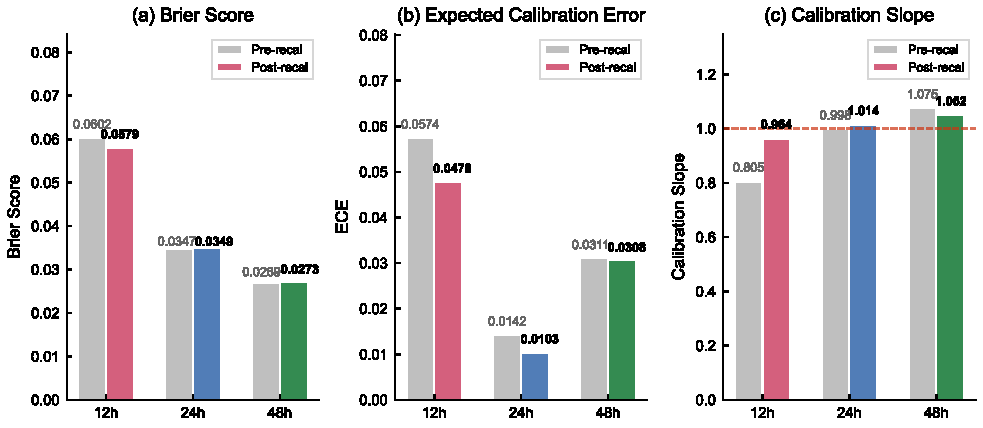
\includegraphics[width=\linewidth]{figures/main/Figure_9_pre_vs_post_recalibration.pdf}
\end{adjustwidth}
    \caption{Pre- vs.\ post-recalibration comparison: (a)~Brier score, (b)~ECE, and (c)~calibration slope. Grey bars represent pre-recalibration values; coloured bars represent post-recalibration values.}\label{fig:recalibration}
\end{figure}

Applying joint post-fusion recalibration brought the 12~h Brier score down from 0.060 to 0.058 and the ECE from 0.057 to 0.048, while pulling the calibration slope from 0.805 up to 0.964---close to the ideal target.
The overall IBS proxy decreased slightly from 0.041 to 0.040.
What matters most is that the 24~h and 48~h calibration were left essentially intact (24~h ECE went from 0.014 to 0.010; 48~h ECE stayed at 0.031).
The legacy 12~h-only variant over-corrected (slope = 1.209) and slightly worsened 24~h and 48~h ECE, which confirms that joint recalibration is the safer route for multi-horizon pipelines.
Because the improvement is modest, we keep recalibration as a sensitivity check rather than folding it into the primary model.

\subsection{Robustness Checks for Validation Bias and Censoring Assumptions}\label{sec:robustness_results}

Since verified wildfire-incident identifiers were not available, we ran auxiliary robustness checks using a lean AFT model.
With proxy incident-grouped cross-validation, mean C-index edged down from 0.9318 $\pm$ 0.0119 (standard stratified CV) to 0.9283 $\pm$ 0.0323 (grouped CV), and mean Brier score climbed from 0.1352 $\pm$ 0.0341 to 0.1541 $\pm$ 0.0761 (Supplementary Table~S8).
The C-index drop was small enough to suggest that massive leakage-driven optimism is unlikely, but the grouped partition did push probability error up and substantially widen fold-to-fold variability.
A leave-one-month-out temporal analysis returned an $N$-weighted mean C-index of 0.935 across the six months with $\geq$10 observations.
The three heaviest fire-season months (Jun--Aug; $n = 33$--70) landed within $C = 0.923$--0.943; the sparser months were more erratic, including a March estimate of $C = 1.000$ that is almost certainly artefactual.

On the censoring side, worst-case/best-case event-rate brackets showed sensitivity ranges of 0.027 at 12~h, 0.113 at 24~h, and 0.249 at 48~h, with the 48~h base event rate stretching from 0.299 to 0.548 under extreme scenarios (Supplementary Table~S9).
Short-horizon estimates are comparatively insulated from censoring assumptions; 48~h estimates are much more exposed.
Figure~\ref{fig:robustness} gathers these diagnostics; full-page versions appear in Supplementary Figures~S2 and~S4.

\begin{figure}[!ht]
\begin{adjustwidth}{-\extralength}{0cm}
    \centering
    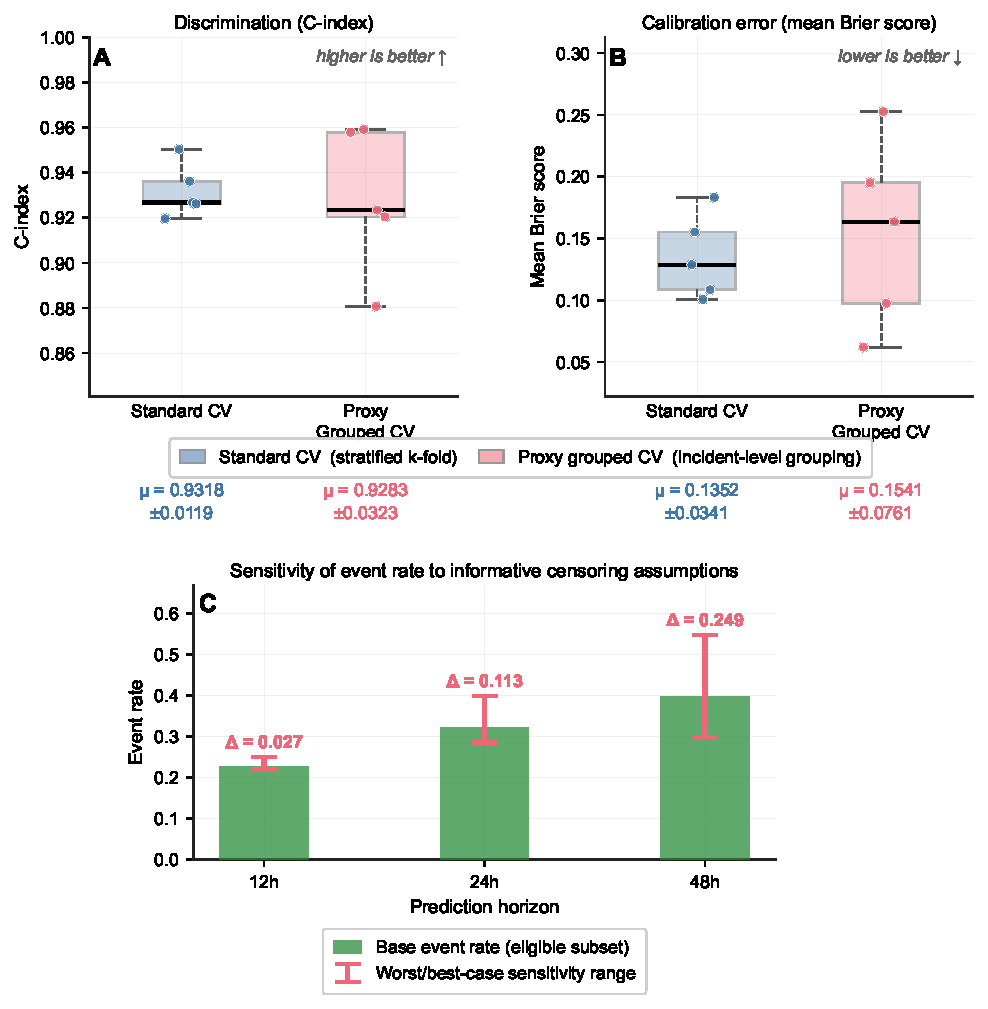
\includegraphics[width=\linewidth]{figures/main/Figure_10_robustness_diagnostics.pdf}
\end{adjustwidth}
    \caption{Main-text robustness diagnostics derived from auxiliary lean-model checks. (a)~Discrimination (C-index) under standard stratified versus proxy incident-grouped cross-validation. (b)~Mean Brier score under the same validation splits, showing worse probability error and greater variability under grouped splitting. (c)~Sensitivity of horizon-specific event rates to informative-censoring assumptions, shown as worst/best-case ranges around the base event rate; the widest range occurs at 48~h. Standalone full-page versions are provided as Supplementary Figures~S2 and~S4.}\label{fig:robustness}
\end{figure}

\subsection{Decision Curve Analysis and Decision Utility}\label{sec:dca_results}

To see how useful the framework's outputs would be for threshold-driven evacuation decisions, we ran a decision curve analysis (DCA)~\cite{Vickers2006} at all three primary horizons.
Table~\ref{tab:dca_utility} lists the decision utility metrics at selected thresholds; net benefit over the full threshold sweep is in Supplementary Table~S5.

\begin{table}[!ht]
\caption{Decision utility at selected probability thresholds (pre-recalibration, nested OOF). Sens.\ = sensitivity; Spec.\ = specificity; PPV = positive predictive value; NPV = negative predictive value; NB = net benefit.}\label{tab:dca_utility}
\small
\begin{tabular}{lccccccc}
\toprule
\textbf{Horizon} & \textbf{Threshold} & \textbf{Sens.} & \textbf{Spec.} & \textbf{PPV} & \textbf{NPV} & \textbf{F1} & \textbf{NB} \\
\midrule
12~h & 0.1 & 0.959 & 0.886 & 0.712 & 0.987 & 0.817 & 0.209 \\
12~h & 0.3 & 0.939 & 0.928 & 0.793 & 0.981 & 0.860 & 0.190 \\
12~h & 0.5 & 0.796 & 0.946 & 0.813 & 0.940 & 0.804 & 0.140 \\
\midrule
24~h & 0.1 & 0.984 & 0.932 & 0.873 & 0.992 & 0.925 & 0.311 \\
24~h & 0.3 & 0.984 & 0.940 & 0.886 & 0.992 & 0.932 & 0.299 \\
24~h & 0.5 & 0.968 & 0.955 & 0.910 & 0.984 & 0.938 & 0.281 \\
\midrule
48~h & 0.1 & 1.000 & 0.950 & 0.930 & 1.000 & 0.964 & 0.394 \\
48~h & 0.3 & 0.985 & 0.950 & 0.929 & 0.990 & 0.956 & 0.379 \\
48~h & 0.5 & 0.970 & 0.960 & 0.941 & 0.980 & 0.955 & 0.361 \\
\bottomrule
\end{tabular}
\end{table}

Across all three horizons the model beat both the ``evacuate every zone'' and ``evacuate no zone'' reference strategies over a wide threshold band.
At 24~h, setting the threshold at 0.3 produced sensitivity of 0.984, specificity of 0.940, and net benefit of 0.299.
The 48~h horizon returned the highest net benefit (0.394 at threshold 0.1), driven by the higher base rate at that window.
Even the 12~h horizon, where calibration is weakest, sustained positive net benefit up to a threshold of roughly 0.8---supporting its use at minimum for relative triage.

\subsection{Feature Importance}\label{sec:feature_importance}

Gain-based feature importance from the AFT backbone (Table~\ref{tab:feature_importance}) confirmed that distance-related variables dominated. Log-distance came first (gain = 20.0), followed by minimum perimeter distance (10.5) and low temporal resolution (8.9).
That distance rules is physically intuitive---closeness to the advancing fire front is, after all, the single strongest predictor of zone-level threat.
The high ranking of temporal resolution and perimeter count is more interesting; it hints that data quality proxies also carry predictive signal, possibly standing in for fire complexity or monitoring intensity.

\begin{table}[!ht]
\caption{Top 10 features by AFT gain-based importance.}\label{tab:feature_importance}
\begin{tabular}{lc}
\toprule
\textbf{Feature} & \textbf{Gain} \\
\midrule
Log-distance              & 20.00 \\
Min distance to perimeter & 10.48 \\
Low temporal resolution   &  8.91 \\
Number of perimeters      &  3.63 \\
Inverse distance          &  3.42 \\
Time span (first--last)   &  2.01 \\
Short-range urgency       &  0.99 \\
Cross-track component     &  0.89 \\
Month (sine)              &  0.73 \\
Start month               &  0.71 \\
\bottomrule
\end{tabular}
\end{table}

\section{Discussion}\label{sec:discussion}

This study examined whether censor-aware survival modelling, multi-horizon calibration, and monotone enforcement can be integrated into a useful framework for wildfire threat-time forecasting. The results suggest that such integration is feasible in principle, although the present dataset places important constraints on the strength of the conclusions. At 221 observations, 69 events (EPV~$\approx$~2.0), and no external validation, the full multi-module architecture did not justify its complexity on aggregate numbers. RSF achieved lower probability error, per-horizon XGBoost showed slightly higher discrimination, and lean AFT variants matched the full model with substantially lower estimation complexity.

Even so, the framework yielded several informative and practically relevant findings. It discriminated well (Uno-C = 0.941), kept Brier scores low (0.027--0.060), and produced well-separated 24~h risk terciles (event rates: 0.0\%, 4.5\%, 92.3\%). The 24~h calibration slope of 0.998 was nearly perfect; at 12~h the model was overconfident (slope = 0.805), which is not unexpected when fire behaviour can pivot so quickly over short intervals; and the 48~h horizon leaned slightly conservative (slope = 1.075) while also being the most exposed to informative-censoring assumptions. These horizon-specific differences have direct operational implications: the 24~h output appears most suitable for absolute threshold-based decisions, the 12~h output is more appropriate for relative zone ranking, and the 48~h output should be interpreted more cautiously.

Two contributions are worth distinguishing. First, the work demonstrates a principled pipeline for producing coherent, cross-horizon threat probabilities under censoring. Second, it provides a practically informative comparison showing that, at the present data scale, simpler censor-aware models---particularly RSF---achieve comparable overall performance. For studies based on similarly limited wildfire encounter datasets, this second finding may be the more immediately actionable one.

\paragraph{Three-tier model roles.}
A useful way to organise the tested models is by complexity tier.
The \emph{full model} occupies the highest complexity tier as a research prototype, integrating survival modelling, horizon-targeted heads, monotone enforcement, and modular ablation for methodological exploration rather than immediate deployment.
The \emph{lean AFT variants} (AFT~+~Cox, AFT~+~Cox~+~Simple) sit in the middle. They retain censor-awareness and monotone coherence while removing much of the additional stacking structure, thereby making the models easier to audit and maintain.
At the lowest end of the complexity spectrum, the \emph{Random Survival Forest} emerged as the strongest practical comparator in this study. RSF combined the lowest IBS (0.032) with the steadiest seed-to-seed behaviour of anything we tested. It handles censoring natively, its CDF-derived probabilities are monotone by construction, and it needs no calibration pipeline at all. What it lacks, relative to our framework, is a modular fusion architecture that can be surgically ablated or extended horizon by horizon.

\paragraph{Framework design and ablation insights.}
The wildfire threat literature has largely focused on two lanes: single-horizon spatial susceptibility mapping~\cite{Jaafari2019,Gigovic2019,Chen2024wui,Kaur2022} and physics-driven spread simulation~\cite{Finney2001,Cruz2003,Shu2020,Pais2021,Zheng2021}. Neither lane produces calibrated, multi-horizon probability outputs that account for censoring.
On the evacuation side, researchers have pursued vulnerability assessments and trigger-point frameworks~\cite{Dolan2022,Paveglio2019,Alcasena2019}; time-to-event perspectives appear occasionally in broader wildfire risk reviews~\cite{Xi2019,Taylor2013}. Still, to our knowledge, no previous study has combined zone-level threat prediction with calibrated multi-horizon output under a formal censoring treatment.

Among the cleaner empirical lessons is that explicit monotone enforcement belongs in any stacked multi-horizon pipeline: roughly a quarter of observations at the 24--48~h boundary had their probabilities out of order before the fusion step fixed them.
The ablation numbers tell a subtler story. Direct heads, grafted onto the AFT backbone alone, actually \emph{degraded} discrimination ($p = 0.024$ for the deficit of AFT~+~Direct relative to the full model), whereas the AFT backbone by itself showed only a non-significant shortfall ($p = 0.340$). The lesson here is architectural: the direct heads inject extra variance that the remaining modules---Cox, gate prior, IPCW, simple distance---must absorb. The modules, in effect, compensate for each other rather than contributing additively.

\paragraph{Module prioritisation under low EPV.}
Pulling together the ablation, lean-variant, and stability evidence, the most sensible reduced architecture at EPV~$\approx$~2.0 is an AFT backbone, optionally paired with the Cox branch (for sharper ranking) and the simple distance head (for anchoring probabilities).
The gate prior, IPCW, and direct heads showed little standalone benefit at this scale; whether they add value at higher event counts is an open question.

\paragraph{Calibration: what each horizon is---and is not---good for.}
The calibration figures in Table~\ref{tab:calibration} need a practical reading.
The 12~h window is inherently volatile---wind shifts, terrain channelling, spot-fire ignition can all redirect a fire within hours. A slope of 0.805 means the model is overconfident at this horizon; relying on a fixed probability cutoff to trigger evacuations at 12~h is therefore risky unless post-fusion recalibration is applied, or the output is restricted to ranking zones rather than making absolute go/no-go calls.
At 24~h the slope of 0.998 is essentially on the money, making this horizon the natural pick for probability-based rules like ``start pre-evacuation staging once $P(T \leq 24) > 0.3$.''
The 48~h slope of 1.075 points to mild conservatism, compounded by the fact that censoring-sensitivity analysis shows the widest event-rate uncertainty at this horizon (range = 0.249). Fire managers should treat 48~h forecasts as rough guidance for advance resource positioning rather than as precise numbers.
There is also a structural factor behind the 12~h pattern: beta calibration targets each base head separately, but the stacking and monotone fusion steps that follow reshape the combined probability distribution. The joint post-fusion temperature scaling we tried brought the 12~h slope back to 0.964 without degrading the other horizons (Table~\ref{tab:recalibration}).

\paragraph{Practical model selection.}
At an EPV of roughly 2.0, the full framework's additional architectural complexity did not convert into significant gains over leaner alternatives ($\Delta$C-index vs.\ AFT-only: $+0.002$, $p = 0.340$; $\Delta$IBS: $-0.002$, $p = 0.390$).
For practical purposes, lean AFT variants are the way to go when modularity matters, and RSF when predictive steadiness is the top priority.

\paragraph{Validation and censoring robustness.}
The proxy incident-grouped cross-validation showed only a modest dip in mean C-index compared with standard stratified CV, which makes it unlikely that leakage from shared incidents inflated the results dramatically. That said, the grouped split did produce worse probability error and much more variable fold-to-fold results.
Temporal blocking told a similar story for the three largest fire-season months (Jun--Aug), but the smaller holdout months were noisier.
Sensitivity to informative censoring widened as the horizon lengthened: the 48~h event-rate estimate could swing anywhere from 29.9\% to 54.8\% under extreme assumptions, which reinforces the view that 24~h is the safest horizon for operational use.

\paragraph{Practical implications.}
The framework's most tangible value probably lies in triage-style risk stratification.
Take a concrete scenario: a wildfire--zone pair 3200~m from the perimeter, fire closing at 400~m/h, area growing at 50~ha/h. The fused outputs would put it at roughly $P(T \leq 12) = 0.72$, $P(T \leq 24) = 0.91$, $P(T \leq 48) = 0.95$---firmly in the high-risk tercile.
The dramatic gap between the 24~h terciles (0.0\% vs.\ 92.3\% observed events) translates naturally into a three-tier protocol: immediate pre-evacuation for high-risk zones, standby for medium-risk, routine monitoring for low-risk. Because this triage relies on ranking ability (C-index = 0.941) rather than on exact probability values, it is more resilient to calibration imperfections than hard-threshold rules.
DCA results support this interpretation: the model showed positive net benefit over a wide threshold range (sensitivity~$>$~0.98, specificity~$>$~0.93 at the 0.3 cutoff for 24~h).
We want to be clear that the framework is a decision-support tool, not a standalone trigger. Any real deployment would need integration with live fire-behaviour data feeds~\cite{Radeloff2023}, validation against agency-specific protocols, and most likely regulatory sign-off.

\paragraph{Strengths and limitations.}
On the strengths side, this study formulates the problem in a censor-aware way, uses nested cross-validation with inner cross-fitting to prevent leakage, and enforces multi-horizon monotonicity. The ablation and baseline comparisons go deeper than is typical in wildfire prediction work, and the lean-variant evaluation together with the five-seed stability check provide secondary guardrails. We also report transparently that simpler alternatives matched or outperformed the full framework---a finding we consider more useful to practitioners than presenting only the favourable numbers.
Future evaluations would benefit from head-to-head comparisons with deep survival architectures (e.g., DeepSurv~\cite{Katzman2018}) and discrete-time hazard models.

Several limitations deserve attention.
First and foremost, the sample ($n = 221$, 69 events, EPV~$\approx$~2.0) is too small to reliably support the full modelling complexity---this alone is the simplest explanation for why the prototype did not outshine simpler competitors~\cite{Riley2020}.
The low EPV also undercuts the stability of three-parameter beta calibration (inner-fold eligible samples as low as $\sim$35), the precision of bootstrap CIs, and the statistical power of ablation tests.
Second, outer-CV folds were not grouped by verified wildfire incident; the proxy grouped-CV analysis pointed to modest average optimism ($\Delta$C-index = $-$0.004), but proper incident-level validation is still needed. We note that the proxy incident-grouped analysis was conducted only on a lean AFT model rather than the full prototype, because applying GroupKFold splitting to the full stacked architecture would have left the inner training folds severely data-starved and rendered cross-fitting unreliable at this sample size.
Third, we did not perform any external spatiotemporal validation.
Fourth, fire containment may breach the independent censoring assumption; worst/best-case event-rate bounds stretched from 0.027 at 12~h to 0.249 at 48~h, arguing for censoring-robust methods or competing-risk formulations going forward.
Fifth, the 72~h horizon was degenerate.
Sixth, both concordance indices and the IBS proxy are approximations chosen for tractability~\cite{Harrell1996,Uno2011,Graf1999}.
Seventh, post-hoc temperature scaling is a sensitivity analysis that introduces its own calibration trade-offs across horizons.
Finally, real-world deployment would demand incident-level and external validation, real-time data integration, and regulatory review.

\section{Conclusions}\label{sec:conclusions}

We built and internally validated a survival--probability fusion framework for multi-horizon wildfire threat forecasting under right censoring. All reported results are based on internal cross-validation of 221 wildfire--zone encounters (69 events). Because no external or incident-grouped validation was performed, the present findings should be interpreted as proof-of-concept evidence rather than as support for operational deployment.

Within those bounds, the framework produced coherent, monotonically ordered probability estimates at 12, 24, and 48~h, with strong discrimination (Uno-C = 0.941) and low probability error (Brier 0.027--0.060). The 24~h horizon came out best calibrated (slope = 0.998) and is the natural choice for absolute threshold-based evacuation triggers. The 12~h horizon is useful for relative zone ranking but less trustworthy for fixed cutoffs (slope = 0.805). The 48~h horizon was mildly conservative and more vulnerable to censoring assumptions---its outputs warrant extra caution. Monotone enforcement fixed incoherent probability sequences in roughly 25\% of observations, confirming that this correction step is not optional in stacked multi-horizon pipelines.

Just as notable is the finding that simpler models performed comparably. RSF delivered lower probability error and tighter seed-to-seed stability; lean AFT variants matched the full model on discrimination while being far easier to implement. At the current data scale (EPV~$\approx$~2.0), a lean AFT pipeline with monotone fusion---or simply an RSF---is the more sensible choice. The full architecture is best understood as a research prototype; whether the additional modules justify their added complexity is a question that can only be settled with substantially larger datasets.

Looking ahead, the priorities are incident-level grouped validation using verified fire identifiers, external spatiotemporal validation spanning diverse fire regimes, and benchmarking against discrete-time hazard and deep survival models~\cite{Katzman2018}. Testing the framework in operational early warning settings, fed by real-time fire-spread data, is the essential next step before any practical deployment.

%=================================================================
% Back Matter
%=================================================================
\vspace{6pt}

\supplementary{The following supporting information is available in the public repository at \url{https://github.com/eee-afkk/wids2026-wildfire-survival}: Table~S0: Complete feature dictionary (name, type, transformation, source). Table~S1: 72~h horizon performance results. Table~S2: Full hyperparameter configurations for all models, including stacking regularisation sensitivity analysis ($\lambda \in \{0.1, 0.5, 1.0, 2.0, 5.0\}$). Table~S3: Two-sided $p$-values for all ablation paired bootstrap comparisons. Table~S4: Fold-level performance metrics (C-index and Brier scores per outer fold). Table~S5: Decision curve analysis net benefit across the full threshold range at 12, 24, and 48~h. Table~S6: Complete feature importance ranking (all features). Table~S7: Practical lean variant comparison with thin-feature configurations. Table~S8: Proxy incident-grouped cross-validation comparison (standard stratified CV vs.\ feature-space clustering GroupKFold; lean AFT model). Table~S9: Informative censoring sensitivity analysis---worst-case/best-case event-rate bounds and Aalen--Johansen competing-risk cumulative incidence by horizon. Table~S10: Leave-one-month-out temporal blocked cross-validation results (lean AFT model). Table~S11: TRIPOD-style data quality summary (missing rates, variable distributions). Figure~S1: Monotonicity verification scatter plots. Figure~S2: Proxy incident-grouped CV comparison---boxplots of C-index and mean Brier score under standard stratified vs.\ grouped cross-validation (43 feature-space proxy groups). Figure~S3: Leave-one-month-out temporal blocked CV---per-month C-index and mean Brier score (months with $n < 10$ excluded); the figure reports unweighted monthly means ($\bar{C} = 0.937$), whereas the main text reports the $N$-weighted mean ($C = 0.935$) to account for differing per-month sample sizes. Figure~S4: Informative censoring sensitivity---worst/best-case event-rate bounds and Kaplan--Meier vs.\ Aalen--Johansen cumulative incidence by horizon. Figure~S5: Kaplan--Meier survival function and event-time vs.\ censoring-time distributions. Figure~S6: Eligible sample size and event rate per prediction horizon. Figure~S7: NIFC WFIGS geographic context---western US wildfire incidents used for supplementary proxy incident grouping (note: the 2026 bar in the annual counts panel may represent a partial year in the downloaded open-data snapshot and should not be interpreted as an anomalous decline). The repository also contains non-numbered workflow support files (e.g., validation\_strategy\_summary.csv) for provenance and navigation; these are not part of the formal supplementary record.}

\authorcontributions{Conceptualization, Z.R.; Methodology, Z.R.; Software, Z.R.; Validation, Z.R.; Formal Analysis, Z.R.; Investigation, Z.R.; Data Curation, Z.R.; Writing---Original Draft Preparation, Z.R.; Writing---Review \& Editing, Z.R.; Visualization, Z.R. The author has read and agreed to the published version of the manuscript.}

\funding{This research received no external funding.}

\institutionalreview{Not applicable.}

\informedconsent{Not applicable.}

\dataavailability{Restrictions apply to the availability of the WiDS Datathon 2026 data used in this study. The data were obtained from the WiDS 2026 Datathon competition platform (\url{https://www.wids.io}) and are available from the provider subject to its terms of access. The analysis code and curated supplementary data files are openly available at \url{https://github.com/eee-afkk/wids2026-wildfire-survival} (DOI to be assigned upon acceptance). Random seeds and environment specifications are documented in the repository README to support reproducibility.}

\conflictsofinterest{The author declares no conflict of interest.}

% AI Usage Disclosure — required by MDPI for manuscripts prepared with AI assistance
\noindent\textbf{AI Tools Disclosure:}
During the preparation of this manuscript, the author used Claude (Anthropic) for English language editing and stylistic polishing of author-written text.
No AI tools were used for study design, data processing, statistical analysis, figure generation, or interpretation of results.
The author reviewed and edited all output and takes full responsibility for the content of the publication.

\abbreviations{The following abbreviations are used in this manuscript:
AFT = Accelerated failure time;
CDF = Cumulative distribution function;
CI = Confidence interval;
DCA = Decision curve analysis;
ECE = Expected calibration error;
ETA = Estimated time of arrival;
GBC = Gradient boosting classifier;
HGB = Histogram gradient boosting classifier;
IBS = Integrated Brier score;
IPCW = Inverse probability of censoring weighting;
LR = Logistic regression;
MCE = Maximum calibration error;
NB = Net benefit;
NPV = Negative predictive value;
OOF = Out-of-fold;
PPV = Positive predictive value;
RSF = Random Survival Forest.
}

%=================================================================
% References — inline thebibliography (MDPI standard, most stable)
%=================================================================
\begin{adjustwidth}{-\extralength}{0cm}
\reftitle{References}

\begin{thebibliography}{99}

\bibitem{Finney2001}
Finney, M.A.
Design of regular landscape fuel treatment patterns for modifying fire growth and behavior.
\textit{For.\ Sci.} \textbf{2001}, \textit{47}, 219--228.

\bibitem{Xi2019}
Xi, D.D.; Taylor, S.W.; Woolford, D.G.; Dean, C.B.
Statistical models of key components of wildfire risk.
\textit{Annu.\ Rev.\ Stat.\ Appl.} \textbf{2019}, \textit{6}, 197--222.

\bibitem{Stephens2018}
Stephens, S.L.; Collins, B.M.; Fettig, C.J.; Finney, M.; Hoffman, C.; Knapp, E.E.; North, M.P.; Safford, H.; Wayman, R.B.
Operational approaches to managing forests of the future in the western United States through complementary fire and forest management strategies.
\textit{For.\ Ecol.\ Manag.} \textbf{2018}, \textit{432}, 987--998.

\bibitem{Jain2022}
Jain, P.; Castellanos-Acuna, D.; Coogan, S.C.P.; Abatzoglou, J.T.; Flannigan, M.D.
Observed increases in extreme fire weather driven by atmospheric humidity and temperature.
\textit{Nat.\ Clim.\ Change} \textbf{2022}, \textit{12}, 63--70.

\bibitem{Cunningham2024}
Cunningham, C.X.; Williamson, G.J.; Bowman, D.M.J.S.
Increasing frequency and intensity of the most extreme wildfires on Earth.
\textit{Nat.\ Ecol.\ Evol.} \textbf{2024}, \textit{8}, 1420--1425.

\bibitem{Turco2023}
Turco, M.; Jerez, S.; Augusto, S.; Tarín-Carrasco, P.; Ratola, N.; Jim\'enez-Guerrero, P.; Trigo, R.M.
Anthropogenic climate change impacts exacerbate summer forest fires in California.
\textit{Proc.\ Natl.\ Acad.\ Sci.\ USA} \textbf{2023}, \textit{120}, e2213815120.

\bibitem{Luo2024}
Luo, K.; Wang, X.; de~Jong, M.; Flannigan, M.
Drought triggers and sustains overnight fires in North America.
\textit{Nature} \textbf{2024}, \textit{627}, 321--327.

\bibitem{Jones2022}
Jones, M.W.; Abatzoglou, J.T.; Veraverbeke, S.; Andela, N.; Lasslop, G.; Forkel, M.; Smith, A.J.P.; Burton, C.; Betts, R.A.; van~der~Werf, G.R.; Sitch, S.; Canadell, J.G.; Sant\'\i n, C.; Kolden, C.; Doerr, S.H.; Le~Qu\'er\'e, C.
Global and regional trends and drivers of fire under climate change.
\textit{Rev.\ Geophys.} \textbf{2022}, \textit{60}, e2020RG000726.

\bibitem{Kolden2024}
Kolden, C.A.; Abatzoglou, J.T.; Jones, M.W.; Jain, P.
Wildfires in 2023.
\textit{Nat.\ Rev.\ Earth Environ.} \textbf{2024}, \textit{5}, 238--240.

\bibitem{Higuera2021}
Higuera, P.E.; Abatzoglou, J.T.
Record-setting climate enabled the extraordinary 2020 fire season in the western United States.
\textit{Glob.\ Change Biol.} \textbf{2021}, \textit{27}, 1--2.

\bibitem{Radeloff2023}
Radeloff, V.C.; Helmers, D.P.; Kramer, H.A.; Mockrin, M.H.; Alexandre, P.M.; Bar-Massada, A.; Butsic, V.; Hawbaker, T.J.; Martinuzzi, S.; Syphard, A.D.; Stewart, S.I.
Rising wildfire risk to houses in the United States, especially in grasslands and shrublands.
\textit{Science} \textbf{2023}, \textit{382}, 702--707.

\bibitem{Tonini2020}
Tonini, M.; D'Andrea, M.; Biondi, G.; Degli Esposti, S.; Ferrari, A.; Pedrazzoli, F.
A machine learning-based approach for wildfire susceptibility mapping: The case study of the Liguria region in Italy.
\textit{Geosciences} \textbf{2020}, \textit{10}, 105.

\bibitem{Cruz2003}
Cruz, M.G.; Alexander, M.E.; Wakimoto, R.H.
Assessing canopy fuel stratum characteristics in crown fire prone fuel types of western North America.
\textit{Int.\ J.\ Wildland Fire} \textbf{2003}, \textit{12}, 39--50.

\bibitem{Jaafari2019}
Jaafari, A.; Zenner, E.K.; Panahi, M.; Shahabi, H.
Hybrid artificial intelligence models based on a neuro-fuzzy network and adaboost algorithm for spatial prediction of wildfire probability.
\textit{J.\ Environ.\ Manag.} \textbf{2019}, \textit{233}, 32--44.

\bibitem{Gigovic2019}
Gigovi\'{c}, L.; Pourghasemi, H.R.; Drobnjak, S.; Bai, S.
Testing a new ensemble model based on SVM and random forest in forest fire susceptibility assessment and its mapping in Serbia's Tara National Park.
\textit{Forests} \textbf{2019}, \textit{10}, 408.

\bibitem{Chen2024wui}
Chen, B.; Jin, Y.; Scaduto, E.; Bhatt, U.; Goulden, M.; Veloz, S.; Moritz, M.
Wildfire risk for global wildland--urban interface areas.
\textit{Nat.\ Sustain.} \textbf{2024}, \textit{7}, 474--484.

\bibitem{Wiegrebe2024}
Wiegrebe, S.; Kopper, P.; Bischl, B.; Bender, A.
Deep learning for survival analysis: A review.
\textit{Artif.\ Intell.\ Rev.} \textbf{2024}, \textit{57}, 65.

\bibitem{Taylor2013}
Taylor, S.W.; Woolford, D.G.; Dean, C.B.; Martell, D.L.
Wildfire prediction to inform fire management: Statistical science challenges.
\textit{Stat.\ Sci.} \textbf{2013}, \textit{28}, 586--615.

\bibitem{VanCalster2019}
Van Calster, B.; McLernon, D.J.; van Smeden, M.; et~al.
Calibration: the Achilles heel of predictive analytics.
\textit{BMC Med.} \textbf{2019}, \textit{17}, 230.

\bibitem{Steyerberg2019}
Steyerberg, E.W.
\textit{Clinical Prediction Models: A Practical Approach to Development, Validation, and Updating}, 2nd~ed.;
Springer: Cham, Switzerland, 2019.

\bibitem{Collins2024}
Collins, G.S.; Moons, K.G.M.; Dhiman, P.; Riley, R.D.; et~al.
TRIPOD+AI statement: updated guidance for reporting clinical prediction models that use regression or machine learning methods.
\textit{BMJ} \textbf{2024}, \textit{385}, e078378.

\bibitem{Riley2020}
Riley, R.D.; Ensor, J.; Snell, K.I.E.; Harrell, F.E.; Martin, G.P.; Reitsma, J.B.; Moons, K.G.M.; Collins, G.; van Smeden, M.
Calculating the sample size required for developing a clinical prediction model.
\textit{BMJ} \textbf{2020}, \textit{368}, m441.

\bibitem{Dolan2022}
Dolan, R.W.; Hammersley, L.A.; McKinley, C.M.
Evacuation trigger assessment for wildfire: A case study.
\textit{Int.\ J.\ Disaster Risk Reduct.} \textbf{2022}, \textit{71}, 102802.

\bibitem{Chen2016}
Chen, T.; Guestrin, C.
XGBoost: A scalable tree boosting system.
In \textit{Proceedings of the 22nd ACM SIGKDD International Conference on Knowledge Discovery and Data Mining};
KDD '16; ACM: New York, NY, USA, 2016; pp.~785--794.

\bibitem{Kull2017}
Kull, M.; Silva Filho, T.; Flach, P.
Beta calibration: A well-founded and easily implemented improvement on logistic calibration for binary classifiers.
In \textit{Proceedings of the 20th International Conference on Artificial Intelligence and Statistics (AISTATS)};
PMLR, 2017; Volume~54, pp.~623--631.

\bibitem{Uno2011}
Uno, H.; Cai, T.; Pencina, M.J.; D'Agostino, R.B.; Wei, L.J.
On the C-statistics for evaluating overall adequacy of risk prediction procedures with censored survival data.
\textit{Stat.\ Med.} \textbf{2011}, \textit{30}, 1105--1117.

\bibitem{Graf1999}
Graf, E.; Schmoor, C.; Sauerbrei, W.; Schumacher, M.
Assessment and comparison of prognostic classification schemes for survival data.
\textit{Stat.\ Med.} \textbf{1999}, \textit{18}, 2529--2545.

\bibitem{Wolpert1992}
Wolpert, D.H.
Stacked generalization.
\textit{Neural Netw.} \textbf{1992}, \textit{5}, 241--259.

\bibitem{VanderLaan2007}
Van der Laan, M.J.; Polley, E.C.; Hubbard, A.E.
Super learner.
\textit{Stat.\ Appl.\ Genet.\ Mol.\ Biol.} \textbf{2007}, \textit{6}, Article~25.

\bibitem{Brier1950}
Brier, G.W.
Verification of forecasts expressed in terms of probability.
\textit{Mon.\ Weather Rev.} \textbf{1950}, \textit{78}, 1--3.

\bibitem{Wolff2019}
Wolff, R.F.; Moons, K.G.M.; Riley, R.D.; et~al.
PROBAST: a tool to assess the risk of bias and applicability of prediction model studies.
\textit{Ann.\ Intern.\ Med.} \textbf{2019}, \textit{170}, 51--58.

\bibitem{Efron1993}
Efron, B.; Tibshirani, R.J.
\textit{An Introduction to the Bootstrap};
Chapman \& Hall: New York, NY, USA, 1993.

\bibitem{Ishwaran2008}
Ishwaran, H.; Kogalur, U.B.; Blackstone, E.H.; Lauer, M.S.
Random survival forests.
\textit{Ann.\ Appl.\ Stat.} \textbf{2008}, \textit{2}, 841--860.

\bibitem{Harrell1996}
Harrell, F.E.; Lee, K.L.; Mark, D.B.
Multivariable prognostic models: Issues in developing models, evaluating assumptions and adequacy, and measuring and reducing errors.
\textit{Stat.\ Med.} \textbf{1996}, \textit{15}, 361--387.

\bibitem{NiculescuMizil2005}
Niculescu-Mizil, A.; Caruana, R.
Predicting good probabilities with supervised learning.
In \textit{Proceedings of the 22nd International Conference on Machine Learning (ICML)};
ACM: New York, NY, USA, 2005; pp.~625--632.

\bibitem{Kaur2022}
Kaur, H.; Bhardwaj, U.
Wildfire risk assessment and prediction: A review.
\textit{Environ.\ Model.\ Assess.} \textbf{2022}, \textit{27}, 381--404.

\bibitem{Shu2020}
Shu, L.; Qu, J.J.; Du, Z.
A review of wildfire spread models.
\textit{Front.\ For.\ China} \textbf{2020}, \textit{15}, 1--12.

\bibitem{Pais2021}
Pais, C.; Carrasco, J.; Martell, D.L.; Weintraub, A.; Woodruff, D.L.
Cell2Fire: A cell-based forest fire growth model.
\textit{Int.\ J.\ Wildland Fire} \textbf{2021}, \textit{30}, 225--237.

\bibitem{Zheng2021}
Zheng, Z.; Huang, W.; Li, S.; Zeng, Y.
Forest fire spread simulating model using a cellular automaton with the effect of topography.
\textit{Simulation} \textbf{2021}, \textit{97}, 387--400.

\bibitem{Paveglio2019}
Paveglio, T.B.; Edgeley, C.M.; Stasiewicz, A.M.
Assessing influences on social vulnerability to wildfire using surveys, spatial data and wildfire simulations.
\textit{J.\ Environ.\ Manag.} \textbf{2019}, \textit{232}, 787--800.

\bibitem{Alcasena2019}
Alcasena, F.J.; Salis, M.; Ager, A.A.; Castell, R.; Vega-Garc\'{\i}a, C.
Assessing wildland fire risk transmission to communities in northern Spain.
\textit{Forests} \textbf{2019}, \textit{10}, 294.

\bibitem{Katzman2018}
Katzman, J.L.; Shaham, U.; Cloninger, A.; Bates, J.; Jiang, T.; Kluger, Y.
DeepSurv: Personalized treatment recommender system using a Cox proportional hazards deep neural network.
\textit{BMC Med.\ Res.\ Methodol.} \textbf{2018}, \textit{18}, 24.

\bibitem{Vickers2006}
Vickers, A.J.; Elkin, E.B.
Decision curve analysis: A novel method for evaluating prediction models.
\textit{Med.\ Decis.\ Making} \textbf{2006}, \textit{26}, 565--574.

\end{thebibliography}
\end{adjustwidth}

\end{document}